\documentclass[10pt,a4paper]{article}
\usepackage[BoldFont,SlantFont,CJKsetspaces,CJKchecksingle]{xeCJK}
\usepackage[dvips]{graphicx}
\setCJKmainfont[BoldFont=SimHei]{Microsoft YaHei}
\setCJKmonofont{Microsoft YaHei}% 设置缺省中文字体
\parindent 2em   %段首缩进
\setlength{\parindent}{22pt}

\author{路少德}

\begin{document}

\begin{center}
  \LARGE{\textbf{《C语言程序设计》课程设计}}
  \newline
  \newline
  \newline
  \huge{\textbf{实验报告}}
  \newline
  \newline
  \newline
  \vspace{4\baselineskip}
  \huge{\textbf{题目:}\underline{伦敦奥运会信息管理系统}}
  \newline
  \Large{专业:\underline{计算机科学与技术~~~}}
  \newline
  \newline
  \Large{班级:\underline{计科1102班\qquad\quad~}}
  \newline
  \newline
  \Large{学号:\underline{u201114166\qquad\qquad}}
  \newline
  \newline
  \Large{姓名:\underline{路少德\qquad\qquad\qquad}}
  \newline
  \newline
  \Large{成绩:\underline{\qquad\qquad\qquad\qquad\quad}}
  \newline
  \newline
  \newline
  \newline
  \Large{指导教师:\underline{曹计昌\qquad\qquad}}
  \newline
  \newline
  \Large{完成日期:\underline{2012年10月14日\qquad\quad}}
\end{center}
\newpage
\tableofcontents
\newpage
\setlength{\parskip}{1ex plus 0.5ex minus 0.2ex}
\section{本系统功能及特色介绍}
\subsection{列表视图}
本系统采用列表视图,将代表团、参赛项目、运动员三级放到界面左侧同一列表下,通过左右方向键进行不同级别链表的切换,同时在右侧显示当前节点的信息,在选中的节点上摁Enter可以进行插入或者修改或者删除等不同的操作,直观便捷。
\subsection{支持Linux系统}
本信息管理系统在Linux下开发完成,弥补Linux平台下因为软件少而可能没有类似软件的缺憾。
\subsection{简洁的界面}
界面采用Ncurses字符终端处理库,所有界面均由作者独立完成,简洁却具备所有功能。键盘操作更快捷。
\subsection{支持中文输入}
本系统在支持英文输入前提下,还支持中文输入和中英文混合输入,方便中国用户。
\subsection{增强用户体验}
本系统开启时自动加载数据文件,退出时如果没有保存还会提示是否保存。另外还可对输入数据进行判断是否合乎规定,避免出错。
\subsection{人性化的查找系统}
本信息管理系统不仅可以通过各级节点的编号查找,还可以通过名称查找,而且只需要对一个输入框输入,系统就可自动判别是编号还是名称而自动查找用户想要的数据
\newpage
\section{题目}
\subsection{题目:伦敦奥运会信息管理系统}
\subsection{需要处理的数据}
\subsubsection{代表团基本信息参考}
\begin{tabular}{|c|c|c|}
  \hline
  中文字段名 &  类型及长度 & 举例\\
  \hline
  代表团编号 & char[6] & 100001 \\
  \hline
  代表团名称 & char[20] & 中国体育代表团 \\
  \hline
  所在国 & char[20] & 中华人民国和国 \\
  \hline
  团长姓名 & char[20] & ~ \\
  \hline
  团长联系方式 & char[20] & ~ \\
  \hline
  参赛运动项目数 & int & ~ \\
  \hline
  参赛运动员数 & int & ~ \\
  \hline
  教练员人数 & int & ~ \\
  \hline
  裁判人数 & int & ~ \\
  \hline
  其他辅助人员人数 & int & ~ \\
  \hline
  代表团入住地址 & char[20] & ~ \\
  \hline
  代表团入住电话 & char[20] & ~ \\
  \hline
  预订房间数 & int & ~ \\
  \hline
  需配备翻译人数 & int & ~ \\
  \hline
  入住奥运村时间 & char[20] & YYYY-MM-DD-HH-MM-SS \\
  \hline
  离开奥运村时间 & char[20] & YYYY-MM-DD-HH-MM-SS \\
  \hline
\end{tabular}

\subsubsection{参赛项目基本信息参考}

\begin{tabular}{|c|c|c|}
  \hline
  中文字段名 & 类型及长度& 举例\\
  \hline
  参赛项目编号 & char[4] & 1005 \\
  \hline
  参赛项目名称 & char[20] & 1005代表男子400米 \\
  \hline
  代表团编号 & char[6] & 100001 \\
  \hline
  项目领队姓名 & char[8] & \\
  \hline
  领队联系方式 & char[20]& \\
  \hline
  教练员人数 & int & \\
  \hline
  参赛运动员人数 & int & \\
  \hline
  历次去的最好成绩 & char[20] & \\
  \hline
  取得最好成绩时间 & char[20] & YYYY-MM-DD-HH-MM-SS \\
  \hline
  取得最好成绩地点 & char[20] & \\
  \hline
  违禁记录 & char[1] & Y有,N无 \\
  \hline
\end{tabular}

\subsubsection{参赛选手基本信息参考}

\begin{tabular}{|c|c|c|}
  \hline
  中文字段名 & 类型及长度& 举例\\
  \hline
  参赛选手编号 & char[8] & \\
  \hline
  参赛项目编号 & char[4] & \\
  \hline
  代表团编号 & char[6] & \\
  \hline
  参赛选手姓名 & char[8] & \\
  \hline
  姓名 & char[1] & M/F \\
  \hline
  出生日期 & char[12] & YYYY-MM-DD \\
  \hline
  出生地 & char[20] & ~ ~ ~中国,湖北,武汉 ~ ~ ~ \\
  \hline
  身高 & int & 182cm\\
  \hline
  体重 & int & 75kg \\
  \hline
  入围成绩 & char[20] & \\
  \hline
    最好成绩 & char[20] & \\ 
  \hline
  兴趣爱好 & char[256] & \\
  \hline
\end{tabular}
\subsection{需实现的系统功能}
\subsubsection{信息录入和插入}
\begin{verbatim}
    * 代表团基本信息录入和插入
    * 参赛项目基本信息录入和插入 
    * 参赛选手基本信息录入和插入 
    * 其他基本信息录入和插入 
\end{verbatim}
\subsubsection{信息修改}
\begin{verbatim}
    * 代表团基本信息修改 
    * 参赛项目基本信息修改 
    * 参赛选手基本信息修改 
    * 其他基本信息修改 
\end{verbatim}
\subsubsection{信息删除}
\begin{verbatim}
    * 代表团基本信息删除 
    * 参赛项目基本信息删除
    * 参赛选手基本信息删除
    * 其他基本信息删除
\end{verbatim}
\subsubsection{信息查询}
\begin{verbatim}
    * 查询指定代表团的团长姓名、参赛运动项目数、参赛运动员人数、代表团入住地地址、入住奥运村时间和离开奥运村时间。
    * 查询某代表团中某参赛项目的领队姓名、参赛运动员人数、历次取得最好成绩,以及是否存在违禁记录信息。
    * 查询某参赛项目的参赛运动员人数最多的领队姓名、代表团名称。
    * 查询指定参赛项目中运动成绩最好的运动员姓名、年龄、身高、体重信息。
\end{verbatim}
\subsubsection{数据统计}
\begin{verbatim}
    * 统计并输出本届奥运会总参赛运动项目数,总参赛运动员人数,总教练员人数,总裁判人数。
    * 统计并输出某指定参赛项目的参赛运动员人数、教练员人数、有违禁记录的代表团数。
    * 统计并输出本届奥运会参赛男女运动员的人数。
    * 统计并输出参赛运动员人数位居前三名的运动项目的名称。
    * 统计并输出本届奥运会体重居前三名运动员姓名,年龄,身高。
\end{verbatim}
\section{系统功能模块结构图}
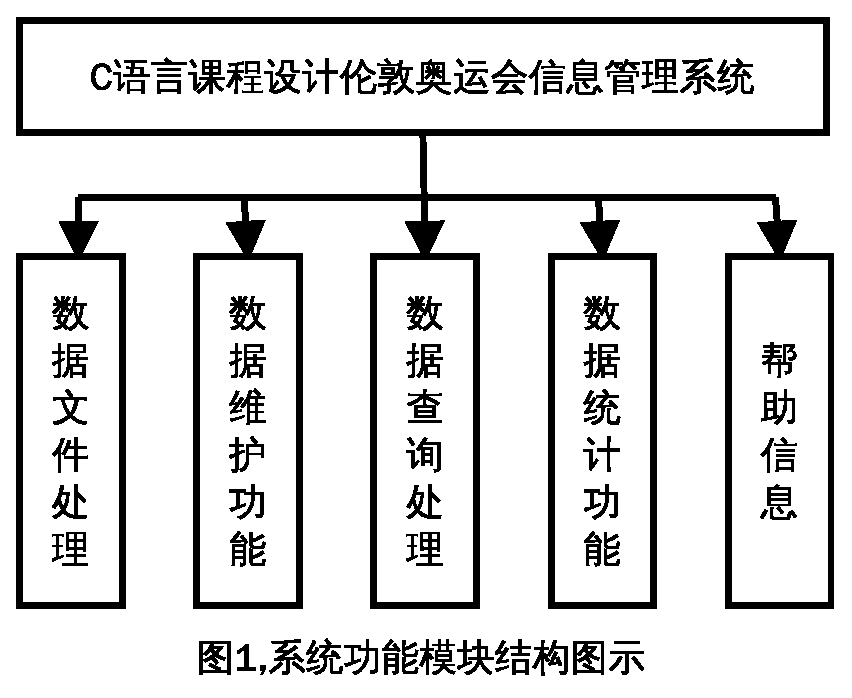
\includegraphics[scale=0.8]{1}
\newline
\newline
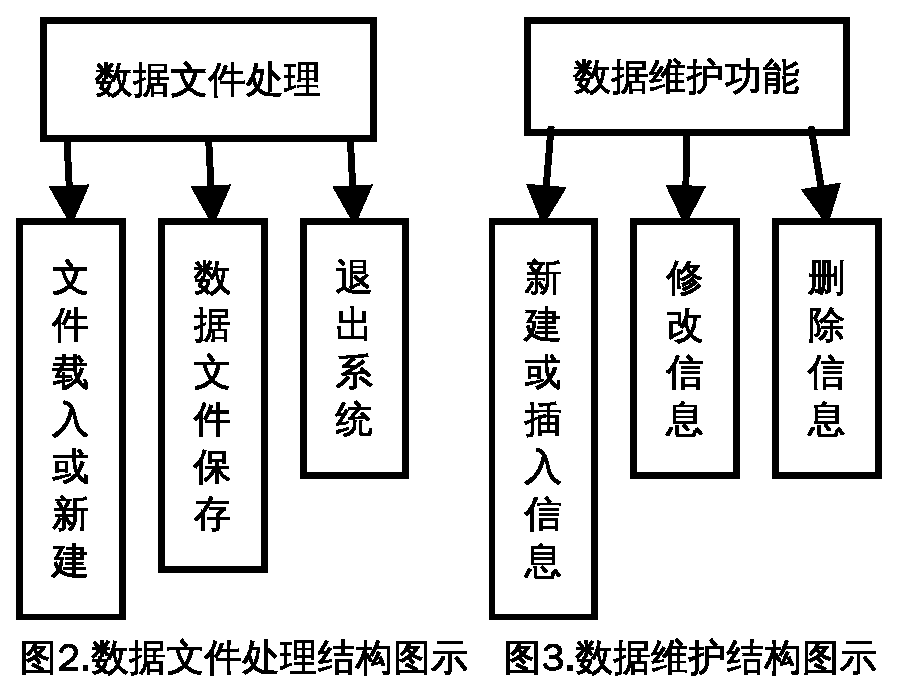
\includegraphics[scale=0.7]{2}
\newline
\newline
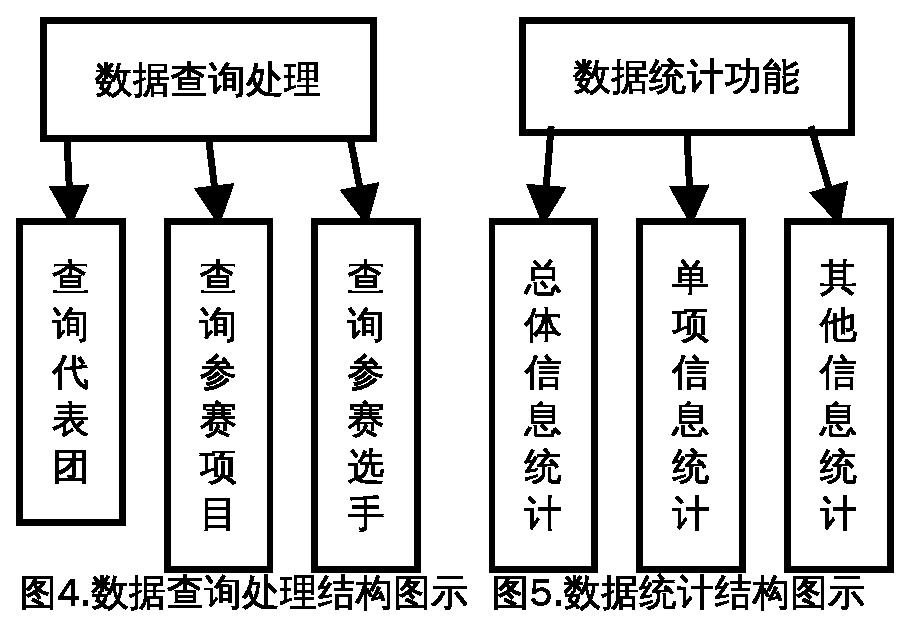
\includegraphics[scale=0.7]{3}
\newline
\newline
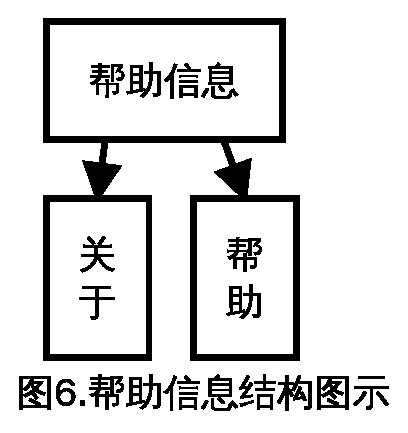
\includegraphics[scale=0.7]{4}
\section{数据结构设计}
\begin{verbatim}
typedef struct _mission {               //代表团结构体
    char index[6+1];                    //代表团编号 
    char name[20+10+1];                 //代表团名称
    char country[20+10+1];              //所在国
    char headerName[20+10+1];           //团长姓名
    char headerContact[20+10+1];        //团长联系方式
    int numSports;                      //参赛运动项目数
    int numSportsman;                   //参赛运动员人数
    int numCoach;                       //教练员人数
    int numJudge;                       //裁判人数
    int numOtherman;                    //其他辅助人员人 
    char address[20+10+1];              //代表团入住地地 
    char telephone[20+10+1];            //代表团入住地电 
    int numRoom;                        //预定房间数
    int numTranslator;                  //需配备翻译人数
    char timeIn[20+10+1];               //入住奥运村时间
    char timeOut[20+10+1];              //离开奥运村时间
    struct _mission* next;              //下一个节点
    struct _entries* headEntries;       //参赛项目头指针
}Mission;
\end{verbatim}
\begin{verbatim}
typedef struct _entries{                //参赛项目结构体
    char index[4+1];                    //参赛项目编号
    char name[20+10+1];                 //参赛项目名称
    char missionIndex[6+1];             //代表团编号
    char leaderName[8+4+1];             //项目领队姓名
    char leaderContact[20+10+1];        //领队联系方式
    int numCoach;                       //教练员人数
    int numSportsman;                   //参赛运动员人数
    char bestAch[20+10+1];              //历次取得最好成绩
    char bestAchTime[20+10+1];          //取得最好成绩时间
    char bestAchLoc[20+10+1];           //取得最好成绩地点
    char isBan;                         //违禁记录        
    struct _entries* next;              //下一个节点      
    struct _sportsman* headSportsman ;  //参赛选手头指针
}Entries;
\end{verbatim}
\begin{verbatim}
typedef struct _sportsman{              //参赛选手结构体
    char index[8+1];                    //参赛选手编号
    char entriesIndex[4+1];             //参赛项目编号 
    char missionIndex[6+1];             //代表团编号
    char name[8+4+1];                   //参赛选手姓 
    char sex;                           //性别
    char birthday[12+1];                //出生日期
    char hometown[20+10+1];             //出生地
    int height;                         //身高
    int weight;                         //体重
    char finalistAch[20+10+1];          //入围成绩
    char bestAch[20+10+1];              //最好成绩
    char hobby[256+1];                  //兴趣爱好     
    struct _sportsman* next;            //下一个节点
}Sportsman;
\end{verbatim}
\section{程序结构(流程图)}
\subsection{软件打开加载流程图}
\begin{center}
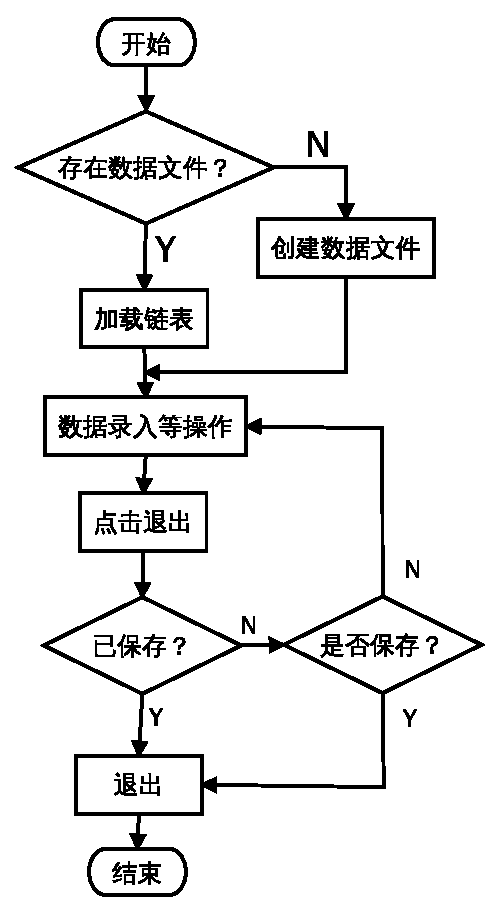
\includegraphics{uml1}
\newline
\end{center}
\subsection{数据查询流程图}
\begin{center}
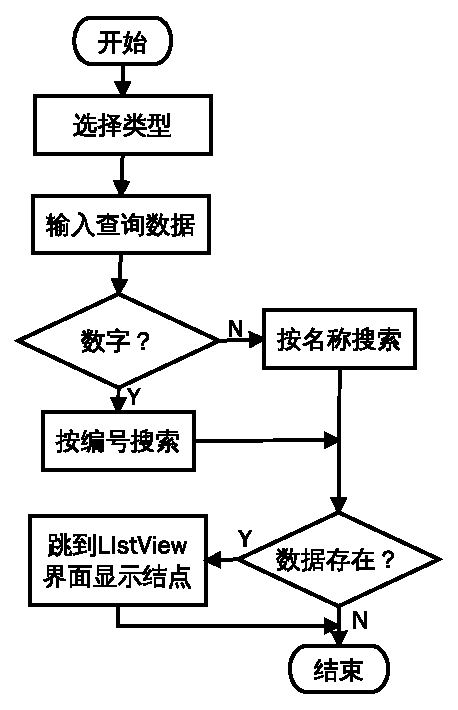
\includegraphics{uml2}
\newline
\end{center}
\section{功能模块及操作说明}
\subsection{打开软件}
在Linux终端下进入本软件所在文件夹,打开本软件。第一次进入会自动在本软件所在文件夹内生成三个文件mission.info,entries.info,sportsman.info以储存数据,以后每次进入都会自动读取文件生成十字交叉链表。
\subsection{保存、清空、退出}
保存和清空时都会进行询问,以确保用户数据的安全性;退出时如果数据没有被修改则不进行询问直接退出,否则询问是否保存。
\subsection{录入与插入信息}
选择 维护->输入->任意一选项 即可进入新建节点的界面,该界面左边是一个ListView,通过上下方向键对节点进行选择,同时右边区域会及时的显示当前节点的信息。最后一个节点是作者设置的空节点以方便保存。通过左右方向键切换链表的等级,右键进入该节点的下一等级的节点,左方向键进入该节点上一等级的节点。在选择好的节点上单击Enter即可进入输入模式,切换到中间的Editbox输入信息,当输入完毕后再摁Enter键进入右边的按钮区进行保存、清空或退出等操作。保存是保存到当前选中的节点之前。
\subsection{修改节点}
修改功能的界面与输入界面一样,区别在于当在保存按钮那里摁Enter键时会将当前选中的节点的信息进行修改。
\subsection{删除节点}
删除功能的界面与输入界面一样,区别在于最后是删除当前节点以及它的所有子节点。
\subsection{查询功能}
当进入查询菜单并且选择对应的查询后,会打开查询窗口,中间有一个输入框,本软件的查询功能可检测用户输入的是字符串还是数字,若是数字则按编号查询,若是字符串则按名称查询。如果查询成功则跳到新建界面的对应节点上,否则弹出没有查询到数据的对话框。
\subsection{统计功能}
统计菜单包含三项 总体、单项、其他,加起来就实现了要求的所有功能。因为其他选项在统计之前要求用户保存文件,所以如果数据被修改的话,会询问是否保存。
\section{试验结果}
7.1 整体界面 \\
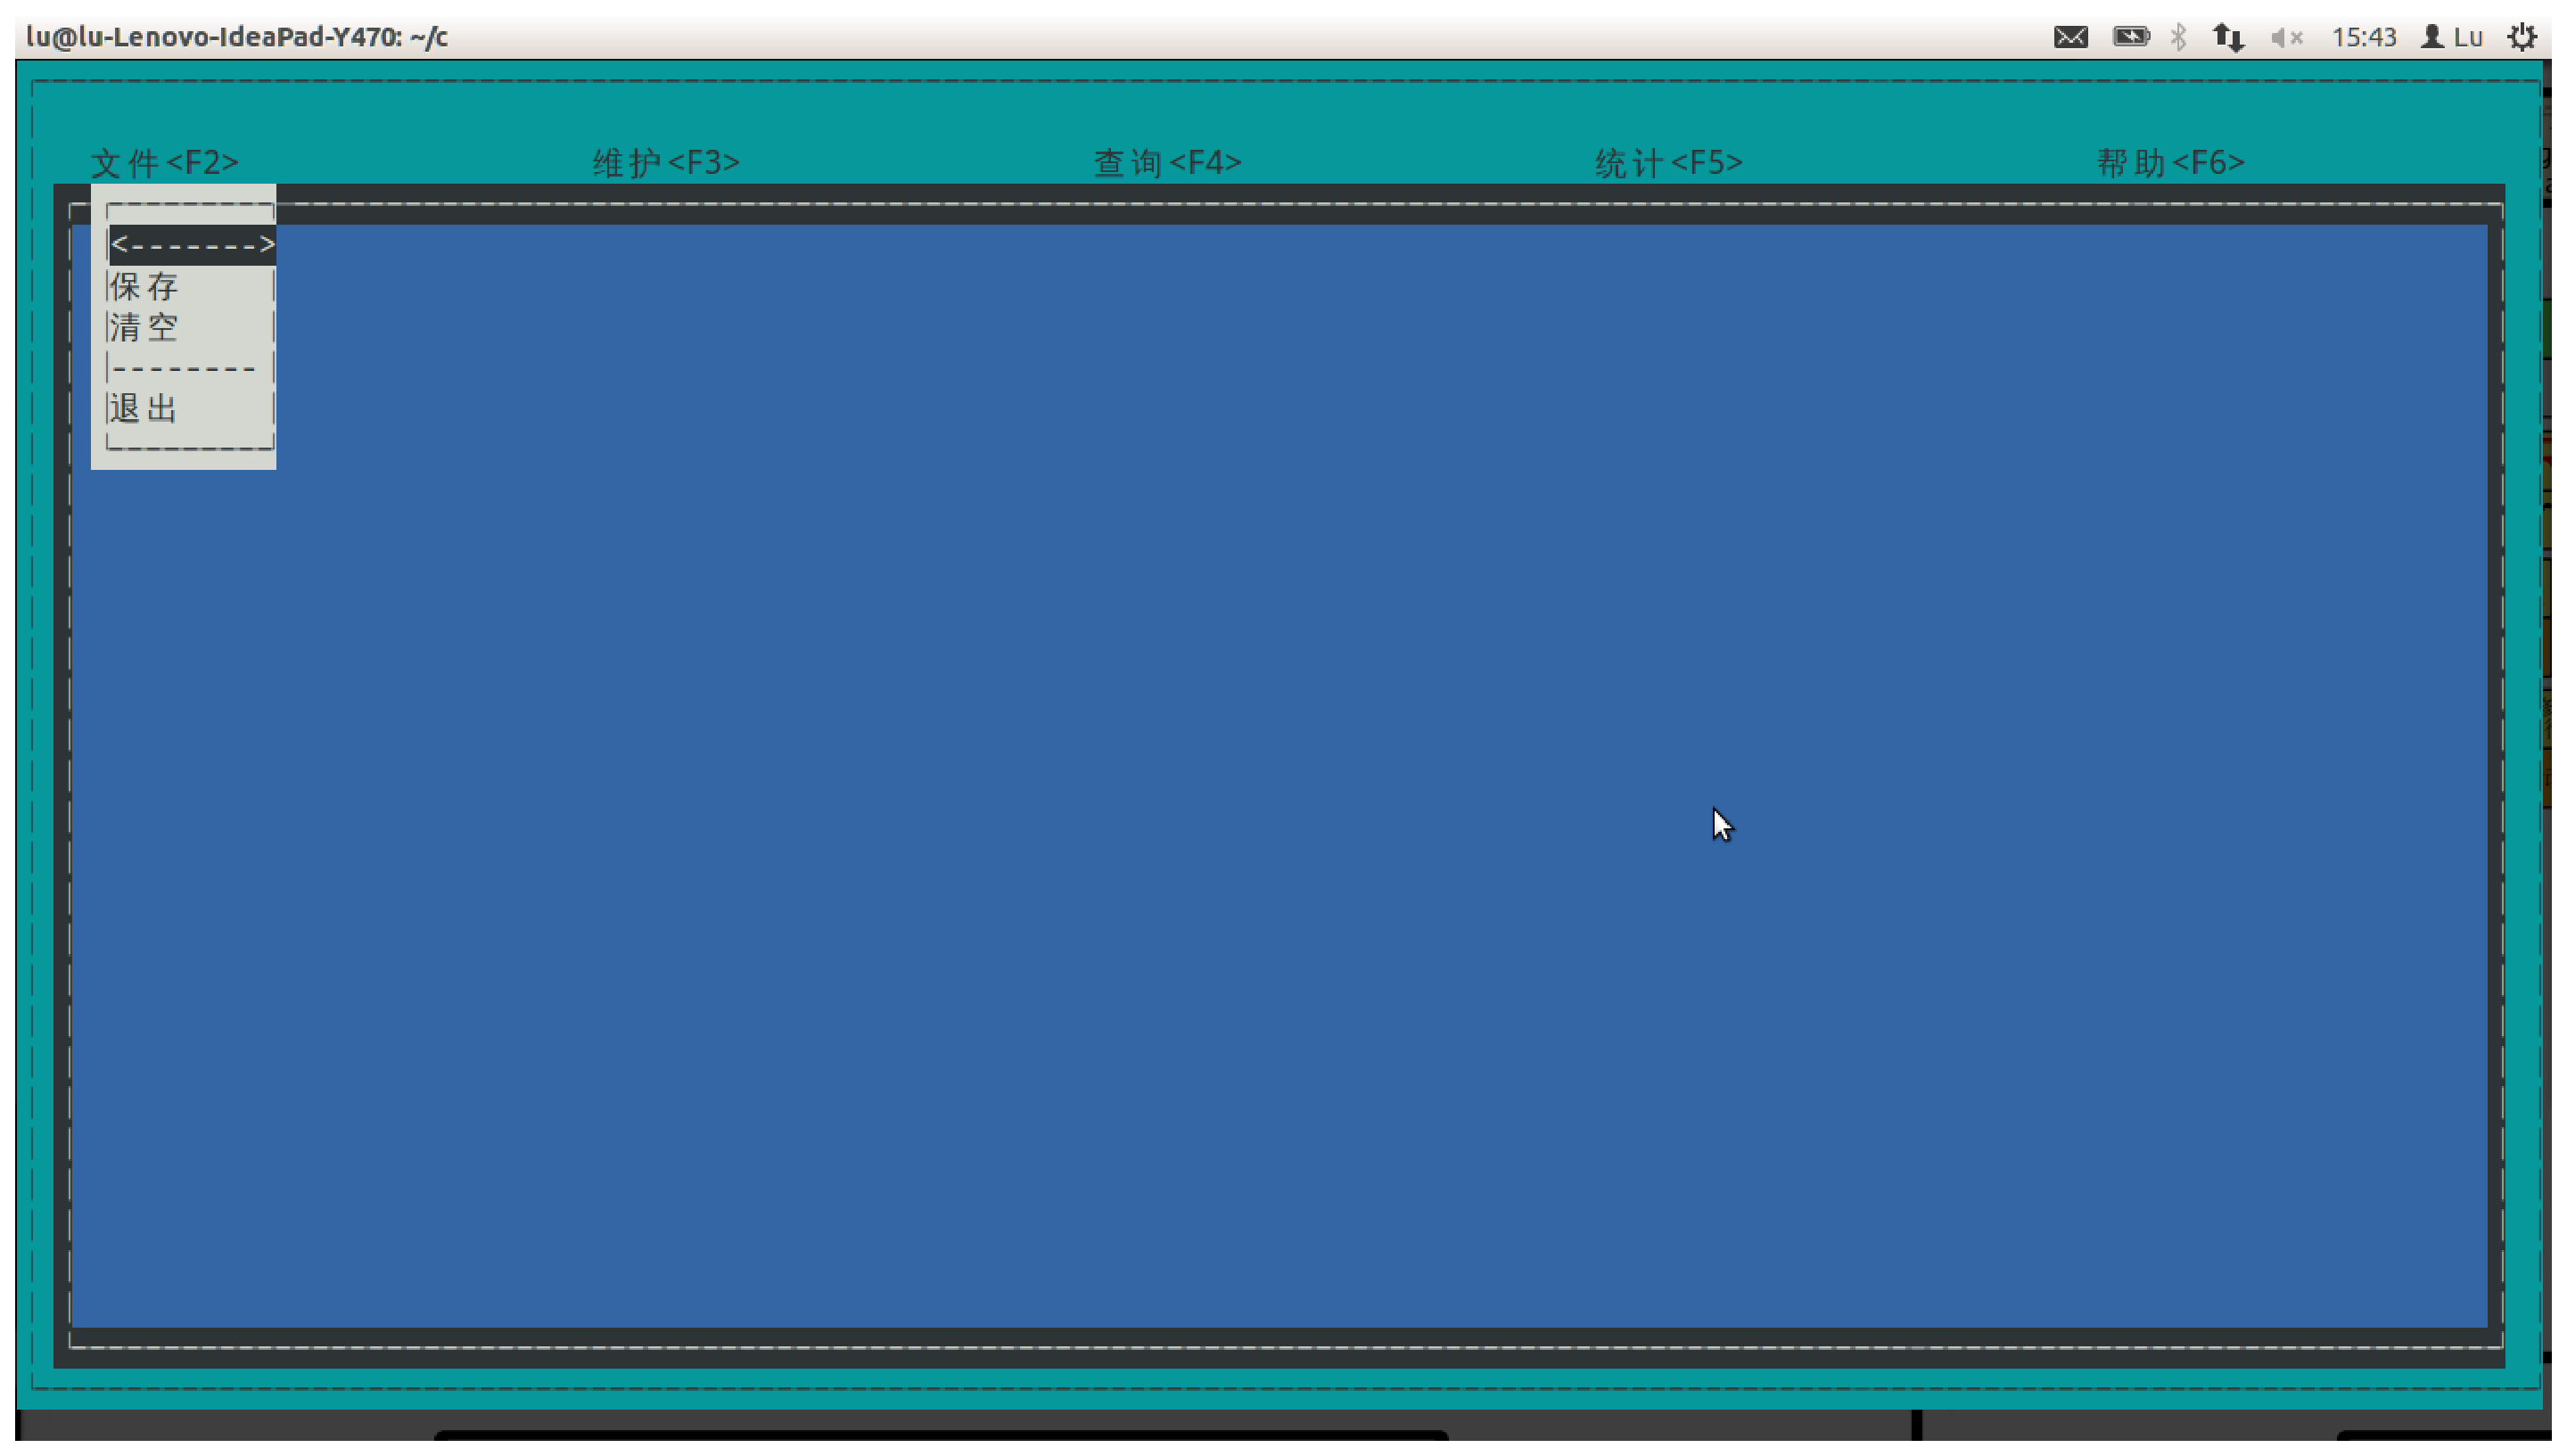
\includegraphics[width=14cm]{p1}
\newline
7.2 保存、清空、退出 \\
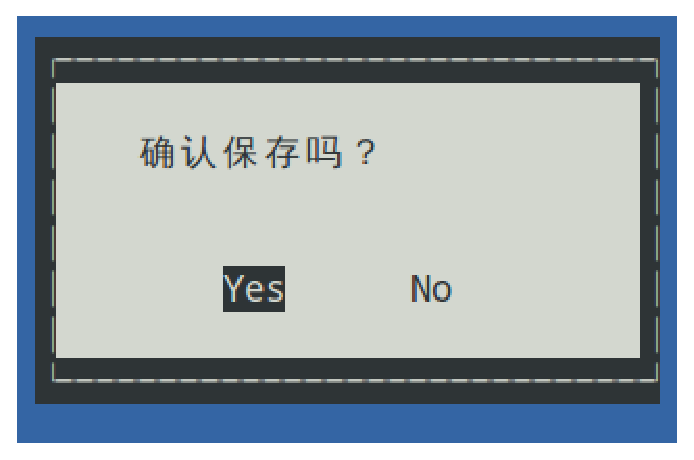
\includegraphics[width=6cm]{save}
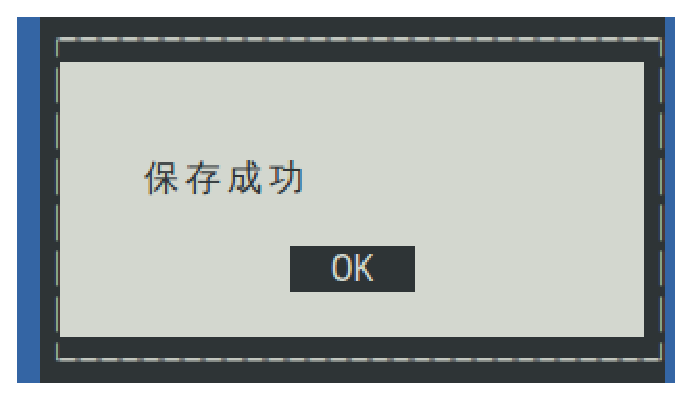
\includegraphics[width=6cm]{saves}
\newline
保存及保存成功
\newline
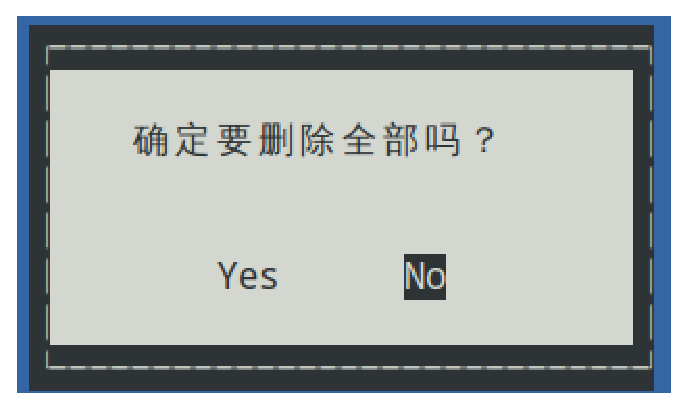
\includegraphics[width=6cm]{clear}
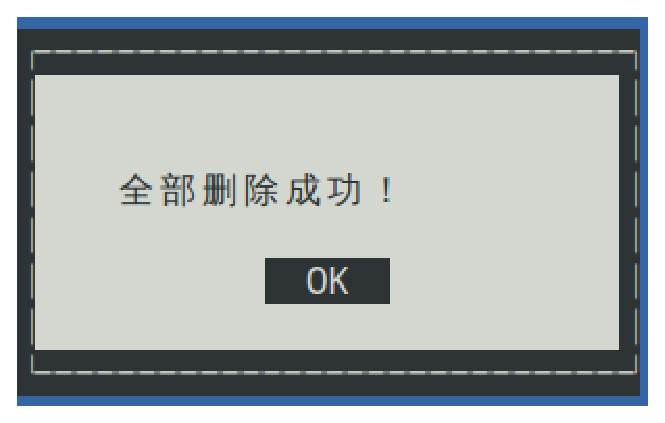
\includegraphics[width=6cm]{clears}
\newline
清空及清空成功
\newline
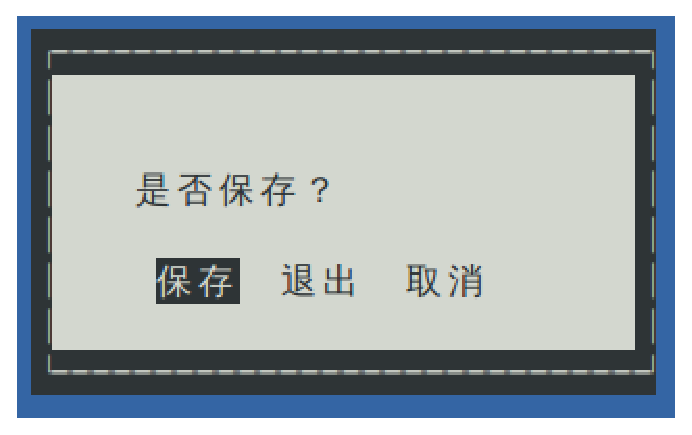
\includegraphics[width=7cm]{exit}
\newline
退出时询问
\newline
7.3 录入与插入信息 \\
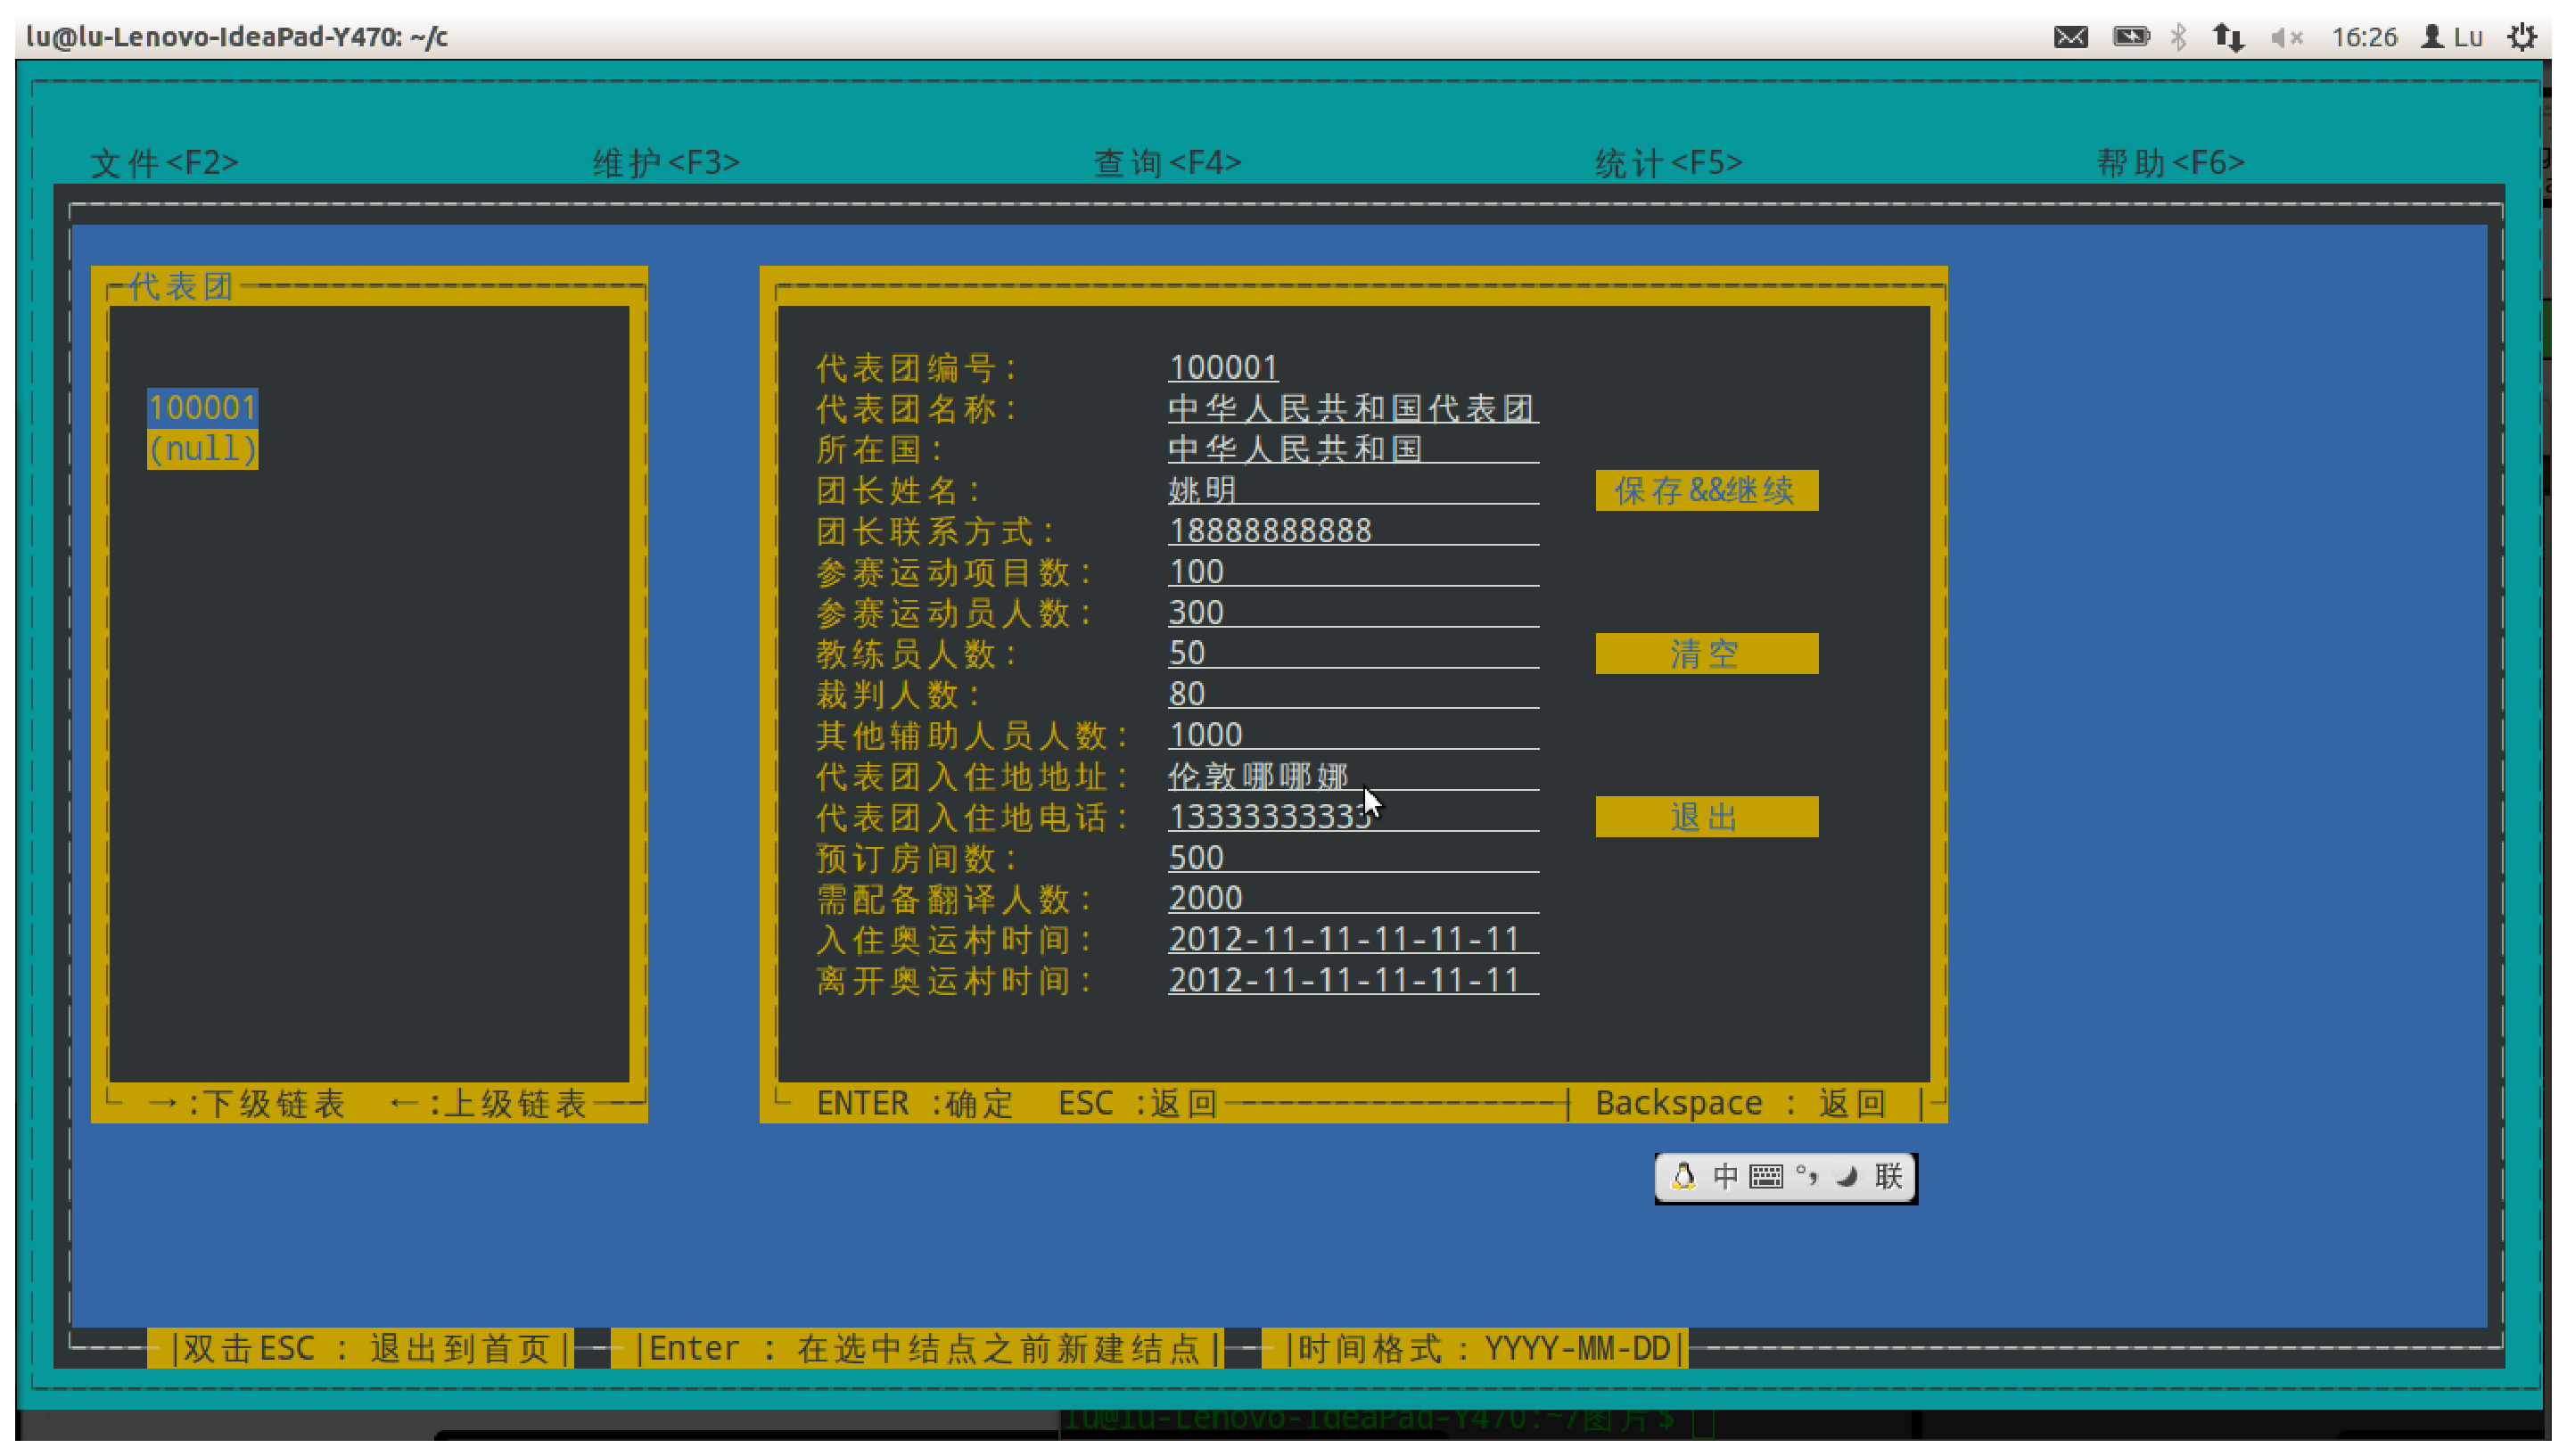
\includegraphics[width=14cm]{addNode}
\newline
整个输入界面
\newline
7.4 修改节点 \\
与添加无太大区别,不再贴图.
7.5 删除节点 \\
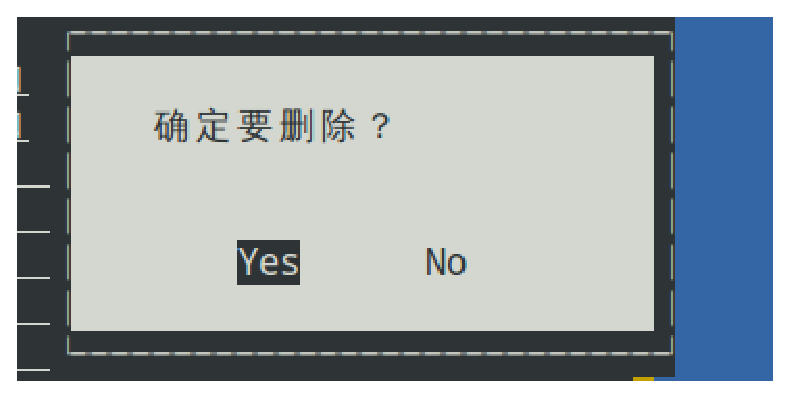
\includegraphics[width=6cm]{delete}
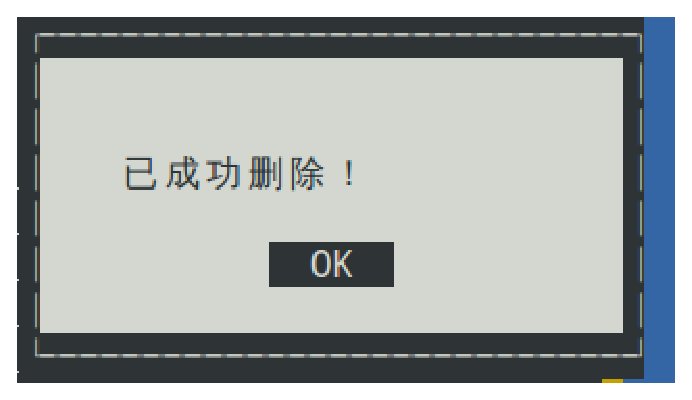
\includegraphics[width=6cm]{deletes}
\newline
删除与删除成功
\newline
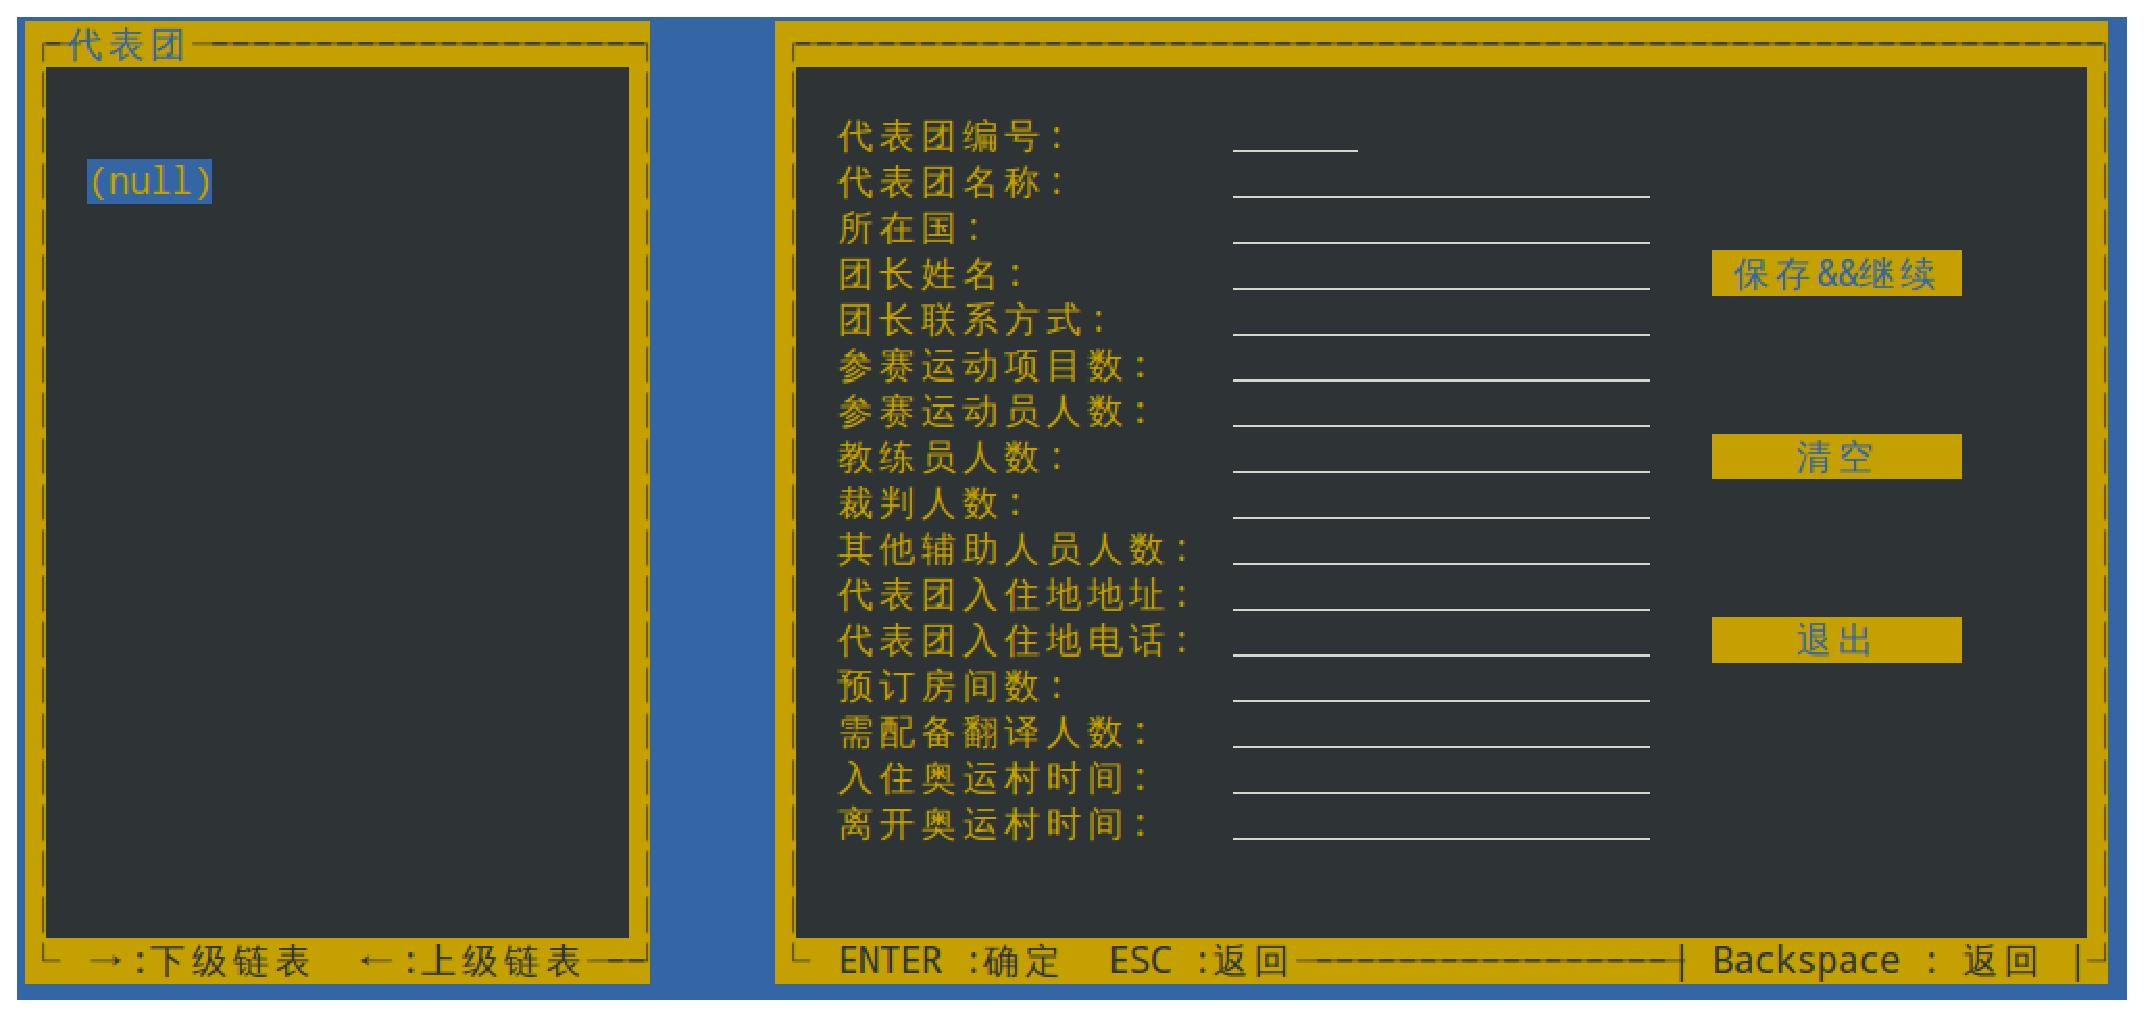
\includegraphics[width=14cm]{deletes1}
\newline
删除成功后的列表
\newline
7.6 查询功能 \\
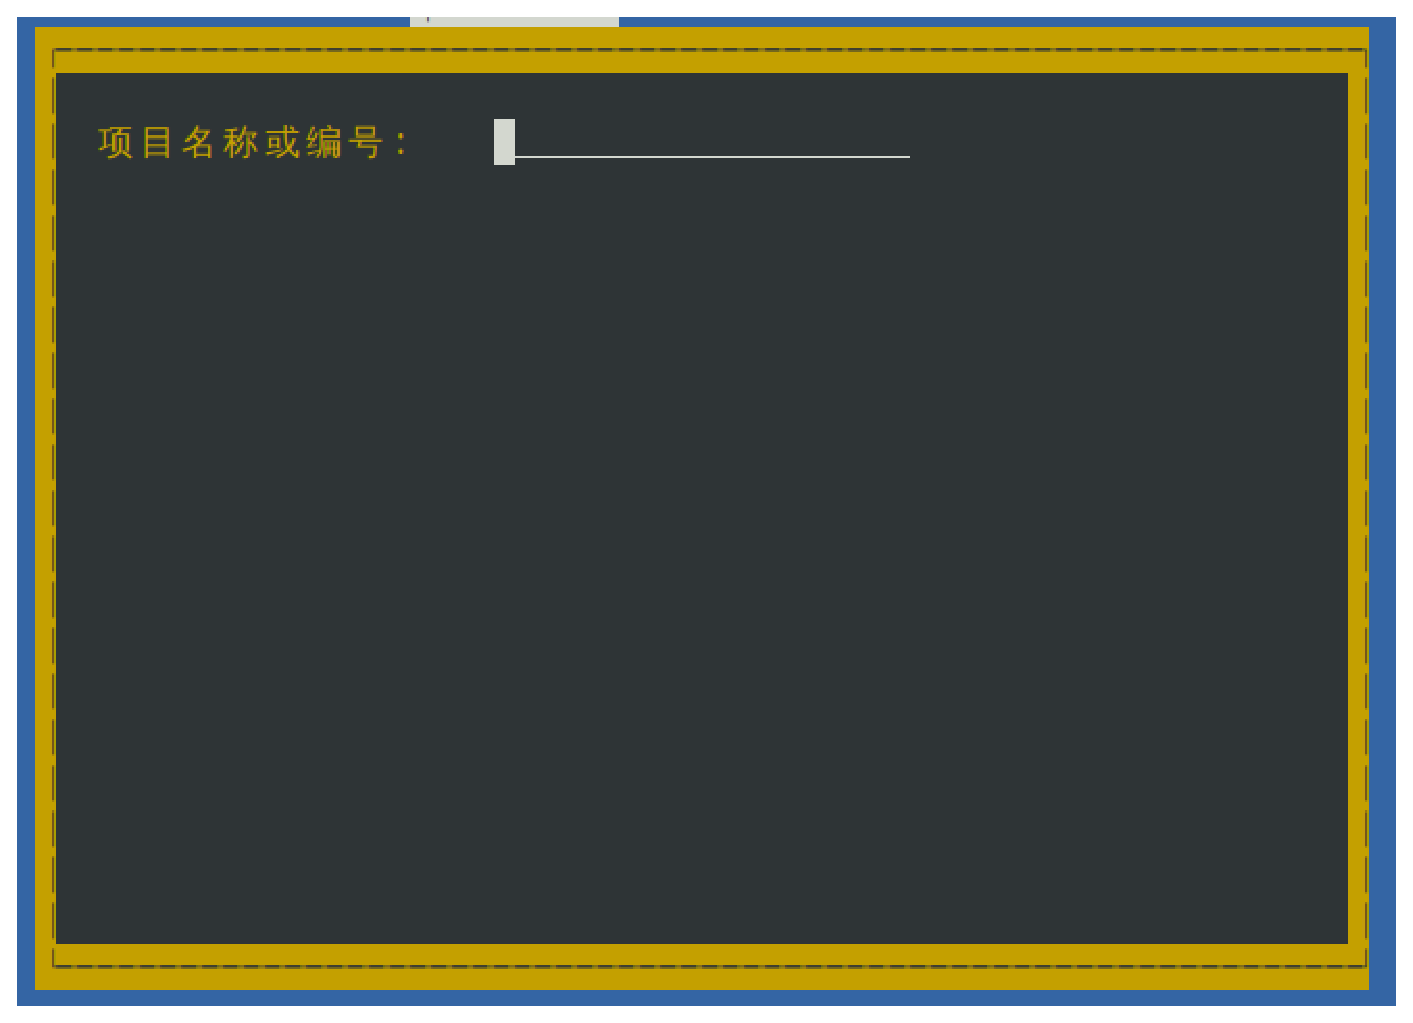
\includegraphics[width=10cm]{query}
\newline
查询界面
\newline
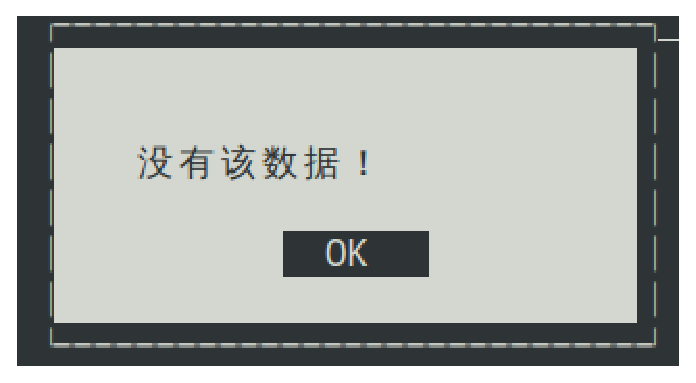
\includegraphics[width=6cm]{queryf}
\newline
没有找到数据对话框
\newline
7.7 统计功能 \\
以下是截图即可清晰的显示每一项的功能。
\newline
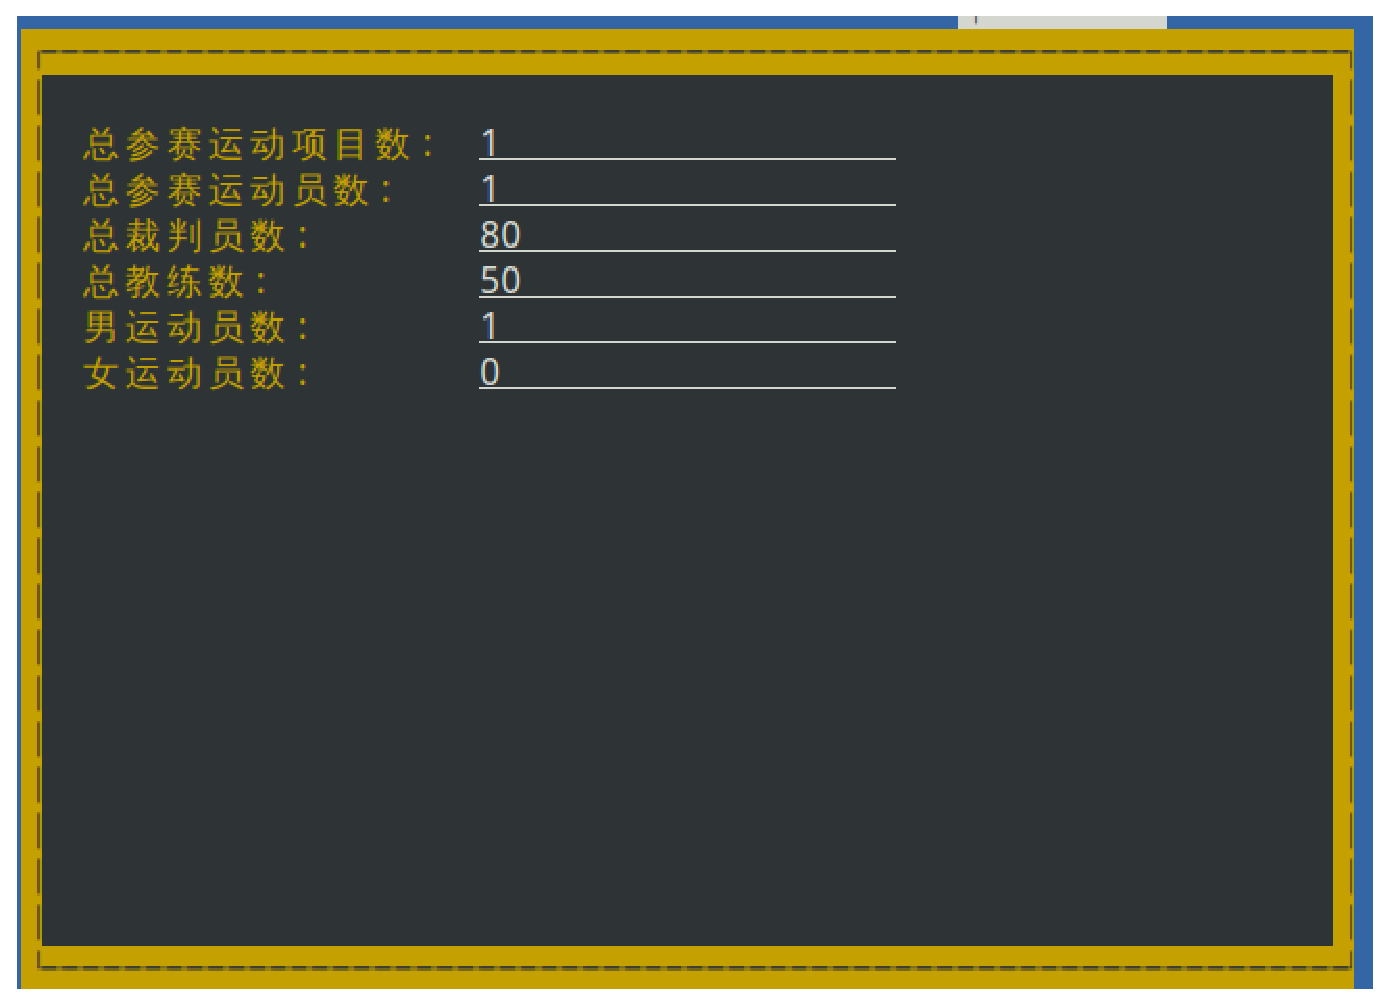
\includegraphics[width=14cm]{staAll}
\newline
统计总体
\newline
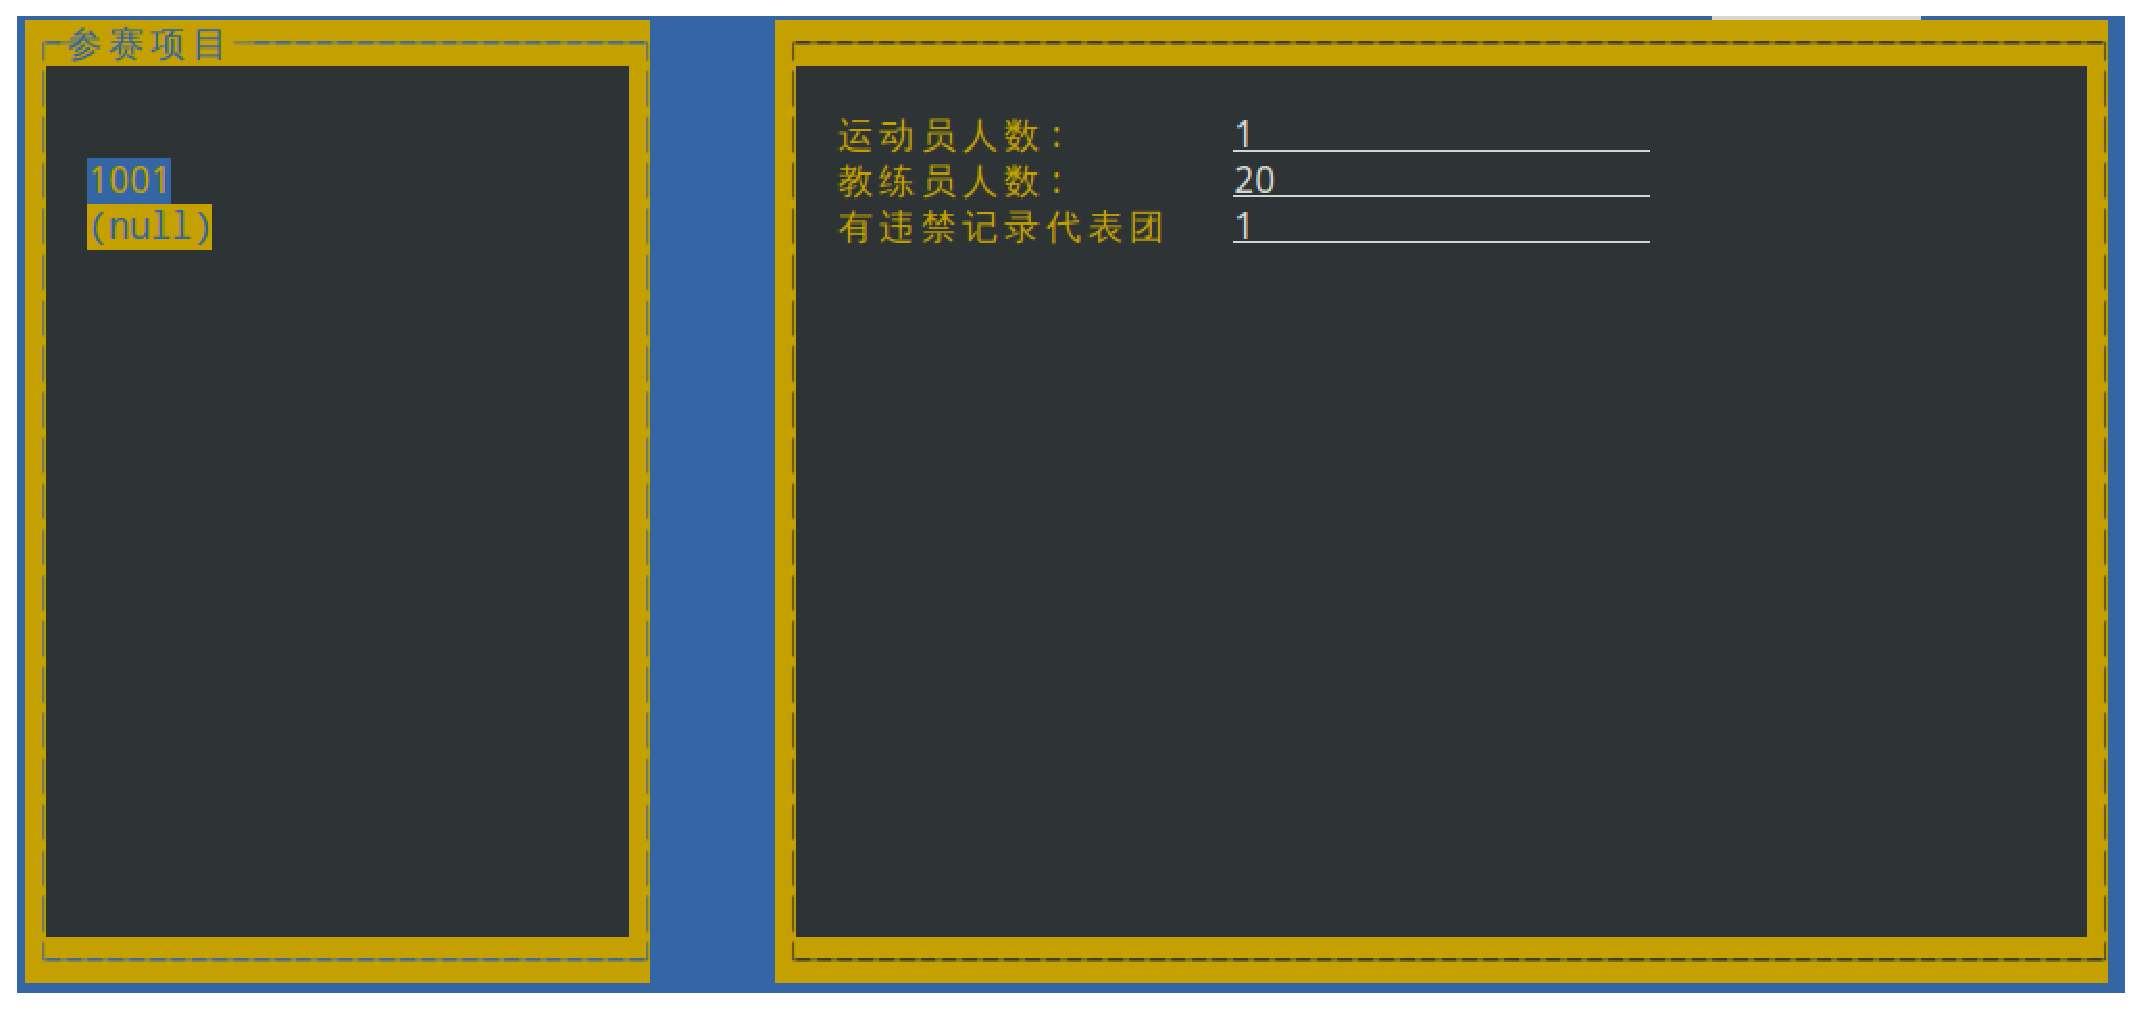
\includegraphics[width=14cm]{staSig}
\newline
统计参赛项目单项
\newline
\includegraphics[width=14cm]{staOth}
\newline
统计其他
\newline
7.8 关于 \\
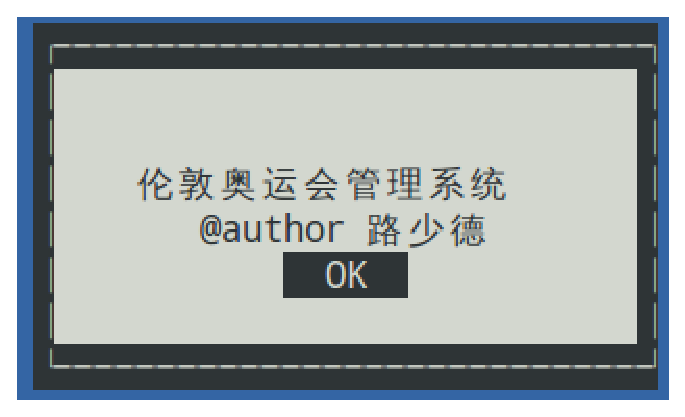
\includegraphics[width=7cm]{about}
\newline
关于界面
\newline

\newpage
\section{体会}
\newpage
\section{附录:程序源代码}
\subsection{前言}
本系统在Linux下用vim编辑完成,用ncurses图形库,Makefile将在下面给出。\\
Makefile使用方法:\\
将3个c文件与一个头文件放在同一目录下,打开终端切换到该目录,输入以下命令:\\
vim Makefile \\
将下面Makefile的内容复制进去: ``+p\\
保存: :wq \\ 
在终端Makefile所在目录下输入 make 即可编译完成。\\
输入 ./main 运行本软件\\
\subsection{Makefile}
\begin{footnotesize}
\begin{verbatim}
main : main.o draw.o list.o
	gcc -o main -Wall -g main.o draw.o list.o -lncursesw -lformw

main.o : main.c drawnlist.h
	gcc -c -g main.c 

draw.o : draw.c drawnlist.h
	gcc -c -g draw.c 

list.o : list.c drawnlist.h
	gcc -c -g list.c 

clean :
	rm edit main.o draw.o list.o
\end{verbatim}
\end{footnotesize}
\begin{footnotesize}
\subsection{main.c}
\begin{verbatim}
#include "drawnlist.h"

int main(int argc, char **argv)
{
    initScreen();       //初始化屏幕
    initColor();        //初始化颜色
    bkgd(COLOR_PAIR(1));//给背景设定颜色
    box(stdscr, 0, 0);  //画边框
    editWin = newwin(LINES-4, COLS-4, 3, 2);
    wbkgd(editWin, COLOR_PAIR(2));
    wattron(editWin, COLOR_PAIR(3));    //当前使用该色彩
    box(editWin, 0, 0);
    wattroff(editWin, COLOR_PAIR(3));   //不使用该色彩了
    wattron(editWin,COLOR_PAIR(7));
    initMenu(); //初始化菜单
    draw_main_menu(stdscr); //画菜单
    initList(); //初始化链表
    while(isOn){
        wnoutrefresh(stdscr);
        wnoutrefresh(editWin);
        doupdate();
        drawMenuList(0, 0);
        touchwin(editWin);
        wrefresh(editWin);
    }
    exitScreen();   //退出函数
    return 0;
}
\end{verbatim}
\subsection{drawnlist.c}
\begin{verbatim}
#include <ncurses.h>	/* stdio.h 也被包含在ncurses.h里面*/
#include <stdlib.h>
#include <string.h>
#include <locale.h>
#include <form.h>

#define MAIN_MENU_NUM	5
#define SUB_MENU_NUM	1
#define KEY_ESC			27
#define ENTER			10
#define MENUNAME_LEN	20
#define MAX_MENU_ITEMS	10

#define NORMAL 0
#define SKIP -1
#define DIALOG -2
#define SAVE -3
#define CREATE -3
#define CREATE_MISSION -30
#define CREATE_ENTRIES -31
#define CREATE_SPORTSMAN -32
#define CHANGE -4
#define CHANGE_MISSION -40
#define CHANGE_ENTRIES -41
#define CHANGE_SPORTSMAN -42
#define DELETE -5
#define DELETE_MISSION -50
#define DELETE_ENTRIES -51
#define DELETE_SPORTSMAN -52
#define STA_ALL -63
#define STA_SINGER -74
#define STA_OTHER -85
#define QUERY -9
#define QUERY_MISSION -96
#define QUERY_ENTRIES -97
#define QUERY_SPORTSMAN -98
#define HELP -10
#define EXIT -'q'

#define ARRAY_SIZE(a) (sizeof(a)/sizeof(a[0]))

struct MenuList {
    char	menuname[MENUNAME_LEN];
    char	str[MAX_MENU_ITEMS][MENUNAME_LEN];
    int		type[MAX_MENU_ITEMS];//正数代表有子菜单且子菜单序号,负数代表其他功能
    int		n;
} menuList[MAIN_MENU_NUM + SUB_MENU_NUM];

/*UTF8中每个汉字3个字节,
 * 因此以下凡是有可能出现汉字的字符串
 * 长度一律×1.5
 */
typedef struct _mission {               //代表团结构体
    char index[6+1];                    //代表团编号 
    char name[20+10+1];                 //代表团名称
    char country[20+10+1];              //所在国
    char headerName[20+10+1];           //团长姓名
    char headerContact[20+10+1];        //团长联系方式
    int numSports;                      //参赛运动项目数
    int numSportsman;                   //参赛运动员人数
    int numCoach;                       //教练员人数
    int numJudge;                       //裁判人数
    int numOtherman;                    //其他辅助人员人 
    char address[20+10+1];              //代表团入住地地 
    char telephone[20+10+1];            //代表团入住地电 
    int numRoom;                        //预定房间数
    int numTranslator;                  //需配备翻译人数
    char timeIn[20+10+1];               //入住奥运村时间
    char timeOut[20+10+1];              //离开奥运村时间
    struct _mission* next;              //下一个结点
    struct _entries* headEntries;       //参赛项目头指针
}Mission;
  
typedef struct _entries{                //参赛项目结构体
    char index[4+1];                    //参赛项目编号
    char name[20+10+1];                 //参赛项目名称
    char missionIndex[6+1];             //代表团编号
    char leaderName[8+4+1];             //项目领队姓名
    char leaderContact[20+10+1];        //领队联系方式
    int numCoach;                       //教练员人数
    int numSportsman;                   //参赛运动员人数
    char bestAch[20+10+1];              //历次取得最好成绩
    char bestAchTime[20+10+1];          //取得最好成绩时间
    char bestAchLoc[20+10+1];           //取得最好成绩地点
    char isBan;                         //违禁记录        
    struct _entries* next;              //下一个结点     
    struct _sportsman* headSportsman ;  //参赛选手头指针
}Entries;
 
typedef struct _sportsman{
    char index[8+1];                    //参赛选手编号
    char entriesIndex[4+1];             //参赛项目编号 
    char missionIndex[6+1];             //代表团编号
    char name[8+4+1];                   //参赛选手姓 
    char sex;                           //性别
    char birthday[12+1];                //出生日期
    char hometown[20+10+1];             //出生地
    int height;                         //身高
    int weight;                         //体重
    char finalistAch[20+10+1];          //入围成绩
    char bestAch[20+10+1];              //最好成绩
    char hobby[256+1];                  //兴趣爱好     
    struct _sportsman* next;
}Sportsman;


extern void initScreen(void);
extern void initColor(void);
extern void initMenu(void);
extern void draw_main_menu(WINDOW *win);
extern void drawMenuList(int m, int t);
extern void moveMenuList(int m, int n);
extern void drawSubmenuList(int m, int n, int k);
extern void moveSubmenuList(int m, int t, int k);
extern void moveMenuItem(int *,int *,int);
extern int doNext(int ,int ,_Bool *);
extern void exitScreen(void);
extern void drawListview(int,int);
extern void createEditbox(int,int,int);
extern int drawButtons(WINDOW**,int,int,int,int type);
extern void cleanFields();
extern void createStaEditbox(int type,int index,int flag);

extern void initList(void);
extern void saveList();

extern Mission* headMission ;
extern Mission* tailMission ;

extern WINDOW	*menu_win[MAIN_MENU_NUM];
extern WINDOW	*sub_win[SUB_MENU_NUM];
extern WINDOW	*editWin;
extern WINDOW   *helpWin;

extern int		screenHeight,screenWidth;
extern int		isOn ;
extern int      isChanged;
extern int		mIndex,eIndex,sIndex;
extern char *info[9][17];
extern char *stringButton[][3];

extern FIELD *fields[17];

extern int addMissionNode(int );
extern int addEntriesNode(int );
extern int addSportsmanNode(int );
extern void delNode(int type);
extern void delMissionNode(Mission* priM);
extern void delEntriesNode(Entries** phE,Entries** priE);
extern void delSportsmanNode(Sportsman** phS,Sportsman** priS);
extern void addMissionInfo(Mission **p);
extern void addEntriesInfo(Entries**);
extern void addSportsmanInfo(Sportsman**);

extern void setMInfo2Fields(Mission *pM);
extern void setEInfo2Fields(Entries *pE);
extern void setSInfo2Fields(Sportsman *pS);
extern void setInfo2Fields(int type);
extern void setIndex2Fields(int type);
extern Mission* fMByIndex();
extern Entries* fEByIndex();
extern Sportsman* fSByIndex();
extern void set2Fields(int type,int flag);
extern void calStaNSet2Fields();
extern void calOthNSet2Fields();
extern void calSigNSet2Fields();
extern int calMSportsmanNum(Mission* pM,int* mN, int* fN);
extern int calESportsmanNum(Entries* pE,int* mN,int* fN);
extern int checkIsStd(int type);
extern int queryGoal(int type,char* name);
extern void deleteAllList();
\end{verbatim}
\end{footnotesize}
\subsection{draw.c}
\begin{footnotesize}
\begin{verbatim}
#include "drawnlist.h"

WINDOW	*menu_win[MAIN_MENU_NUM];//一级子菜单窗口
WINDOW	*sub_win[SUB_MENU_NUM];//二级子菜单窗口
WINDOW	*editWin;//主界面

FIELD *fields[17];//输入框

int		screenHeight,screenWidth;//屏幕高度,宽度
int		isOn = 1;
//三个级别的菜单的标号,-1代表不是当前菜单
int		mIndex = 0,eIndex = -1,sIndex = -1;
int shortcutsF(int);//F(n)快捷键
int getFieldLength(int type,int i);//定义文本域长度
void changeMESIndex(int uod,int size);//改变List标号
int drawSelDialog(char* str,int index);//绘画选择对话框
void drawOKDialog(char* str);//绘画通知对话框
void createStaEditbox(int type,int index,int flag);
int getFieldsNum(int type);
void initFields(WINDOW* formWin,int type);
void drawStaListview(int type,int typeindex,int index);
void createQueryEditbox(int type);
int drawSaveDialog(void);
void createHelpEditbox();

/*各种名称*/
char *info[9][17]={//代表团,参赛项目,运动员
    {//16+1
        "代表团编号",
        "代表团名称",
        "所在国",
        "团长姓名",
        "团长联系方式",
        "参赛运动项目数",
        "参赛运动员人数",
        "教练员人数",
        "裁判人数",
        "其他辅助人员人数",
        "代表团入住地地址",
        "代表团入住地电话",
        "预订房间数",
        "需配备翻译人数",
        "入住奥运村时间",
        "离开奥运村时间",
        (char *)NULL,
    },
    {//11+1
        "参赛项目编号",
        "参赛项目名称",
        "代表团编号",
        "项目领队姓名",
        "领队联系方式",
        "教练员人数",
        "参赛运动员人数",
        "历次去的最好成绩",
        "去的最好成绩时间",
        "去的最好成绩地点",
        "违禁记录",
        (char *)NULL,
    },
    {//12+1
        "参赛选手编号",
        "参赛项目编号",
        "代表团编号",
        "参赛选手姓名",
        "性别",
        "出生日期",
        "出生地",
        "身高",
        "体重",
        "入围成绩",
        "最好成绩",
        "兴趣爱好",
        (char *)NULL,
    },
    {//6+1
        "总参赛运动项目数", 
        "总参赛运动员数",
        "总裁判员数",
        "总教练数",
        "男运动员数",
        "女运动员数",
        (char *)NULL,
    },
    {//3+1
        "运动员人数",  
        "教练员人数",
        "有违禁记录代表团数",
        (char*)NULL,
    },
    {//2+1
        "运动项目人数排名", 
        "",
        "",
        "运动员体重排名",
        "",
        "",
        (char *)NULL,
    },
    {
        "代表团名称或编号", 
        (char *)NULL,
    },
    {
        "项目名称或编号", 
        (char *)NULL,
    },
    {
        "运动员名称或编号", 
        (char *)NULL,
    },
};

/*button的名称*/
char *stringButton[][3]={
    {
        " 保存&&继续 ",
        "    清空    ",
        "    退出    ",
    },
    {
        "   新建   ",
        "   修改   ",
    }
};

/*初始化屏幕*/
void initScreen(void)
{
    setlocale(LC_ALL,"");//使支持utf-8
    initscr();	//初始化ncurses
    noecho();	//输入的字符不可见
    cbreak();	//直接被利用
    getmaxyx(stdscr,screenHeight,screenWidth);//获取屏幕高宽
    start_color();
    curs_set(0);//使光标隐藏
}

/*初始化各种颜色*/
void initColor(void)
{
    init_pair(1, COLOR_BLACK, COLOR_CYAN);
    init_pair(2, COLOR_CYAN, COLOR_BLUE);
    init_pair(3, COLOR_WHITE, COLOR_BLACK);
    init_pair(4, COLOR_BLACK, COLOR_WHITE);
    init_pair(5, COLOR_GREEN, COLOR_BLACK);
    init_pair(6, COLOR_BLUE, COLOR_YELLOW);
    init_pair(7 ,COLOR_BLACK, COLOR_YELLOW);
}

/*
 *setMenuText
 * */
void initMenu(void)
{
    int		i;
    for (i = 0; i < MAIN_MENU_NUM; ++i)
        menu_win[i] = NULL;
    for (i = 0; i < SUB_MENU_NUM; ++i)
        sub_win[i] = NULL;
    strcpy(menuList[0].menuname, "文件<F2>");
    strcpy(menuList[0].str[0],"<------->");
    strcpy(menuList[0].str[1], "保存");
    menuList[0].type[1] = SAVE;
    strcpy(menuList[0].str[2], "清空");
    menuList[0].type[2] = DELETE;
    strcpy(menuList[0].str[3], "--------");
    menuList[0].type[3] = SKIP;
    strcpy(menuList[0].str[4], "退出");
    menuList[0].type[4] = EXIT;
    menuList[0].n = 5;

    strcpy(menuList[1].menuname, "维护<F3>");
    strcpy(menuList[1].str[0],"<------->");
    strcpy(menuList[1].str[1], "输入 ->");
    menuList[1].type[1] = 1;
    strcpy(menuList[1].str[2], "修改");
    //	menuList[1].type[2] = 3;
    menuList[1].type[2] = CHANGE_MISSION;
    strcpy(menuList[1].str[3],"删除");
    //  menuList[1].type[3] = 4;
    menuList[1].type[3] = DELETE_MISSION;
    menuList[1].n = 4;

    strcpy(menuList[2].menuname, "查询<F4>");
    strcpy(menuList[2].str[0],"<------->");
    strcpy(menuList[2].str[1], "代表团");
    menuList[2].type[1] = QUERY_MISSION;
    strcpy(menuList[2].str[2], "项目");
    menuList[2].type[2] = QUERY_ENTRIES;
    strcpy(menuList[2].str[3], "运动员");
    menuList[2].type[3] = QUERY_SPORTSMAN;
    menuList[2].n = 4;

    strcpy(menuList[3].menuname, "统计<F5>");
    strcpy(menuList[3].str[0],"<------->");
    strcpy(menuList[3].str[1], "总体");
    menuList[3].type[1] = STA_ALL;
    strcpy(menuList[3].str[2], "单项");
    menuList[3].type[2] = STA_SINGER;
    strcpy(menuList[3].str[3],"其他");
    menuList[3].type[3] = STA_OTHER;
    menuList[3].n = 4;

    strcpy(menuList[4].menuname, "帮助<F6>");
    strcpy(menuList[4].str[0],"<------->");
    strcpy(menuList[4].str[1], "关于");
    menuList[4].type[1] = -2;
    strcpy(menuList[4].str[2], "帮助");
    menuList[4].type[2] = HELP;
    menuList[4].n = 3;

    //以下是子菜单
    strcpy(menuList[5].str[0], "代表团");
    menuList[5].type[0] = CREATE_MISSION;
    strcpy(menuList[5].str[1], "项目");
    menuList[5].type[1] = CREATE_ENTRIES;
    strcpy(menuList[5].str[2], "运动员");
    menuList[5].type[2] = CREATE_SPORTSMAN;
    menuList[5].n = 3;
}

/*画主菜单*/
void draw_main_menu(WINDOW *win)
{
    int		i;
    for (i = 0; i < MAIN_MENU_NUM; ++i)
        mvwprintw(win, 2, 4+i*screenWidth/5, menuList[i].menuname);
}

/*!
  画一级子菜单
  \param m:主菜单第m项 t:子菜单第t项
  */
void drawMenuList(int m, int t)
{
    int		i;
    curs_set(0);
    wattron(editWin, COLOR_PAIR(3));
    box(editWin, 0, 0);
    wattroff(editWin, COLOR_PAIR(3));
    if (NULL == menu_win[m]) {
        menu_win[m] = newwin(2+menuList[m].n, 10, 3, 4+m*screenWidth/5);
        wbkgd(menu_win[m], COLOR_PAIR(4));
    }

    touchwin(editWin);
    wrefresh(editWin);
    box(menu_win[m], 0, 0);

    //画各项,选中的反色显示
    for (i = 0; i < menuList[m].n; ++i) {
        if (t == i) wattron(menu_win[m], A_REVERSE);
        mvwprintw(menu_win[m], i+1, 1, menuList[m].str[i]);
        if (t == i) wattroff(menu_win[m], A_REVERSE);
    }
    wrefresh(menu_win[m]);
    moveMenuList(m, t);//进入监听
    delwin(menu_win[m]);
}

/*!
  在一级子菜单下对键盘的监听
  \param m:主菜单第m项 t:子菜单第t项
  */
void moveMenuList(int m, int t)
{
    int		ch;
    bool	bdomenu = TRUE;

    keypad(menu_win[m], TRUE);
    while (bdomenu) {
        ch = wgetch(menu_win[m]);
        //对快捷键F(n)判断
        if((shortcutsF(ch))) bdomenu =FALSE;
        switch (ch) {
            case KEY_ESC:
                drawMenuList(m, 0);
                bdomenu = FALSE;
                break;
            case 'q':
                drawMenuList(0, 5);
                bdomenu = FALSE;
                break;
            case KEY_LEFT:
                drawMenuList((m+MAIN_MENU_NUM-1)%MAIN_MENU_NUM, 0);
                bdomenu = FALSE;
                break;
            case KEY_RIGHT:
                //有子菜单则画出子菜单,否则往右移动
                if(menuList[m].type[t]>0){
                    drawSubmenuList(m, t, MAIN_MENU_NUM+menuList[m].type[t]-1);
                    drawMenuList(m, 0);
                } else{
                    drawMenuList((m+MAIN_MENU_NUM+1)%MAIN_MENU_NUM, 0);
                }

                bdomenu = FALSE;
                break;
            case KEY_UP:
                mvwprintw(menu_win[m], t+1, 1, menuList[m].str[t]);
                t = (t+menuList[m].n-1)%menuList[m].n;
                moveMenuItem(&m,&t,-1);
                wattron(menu_win[m], A_REVERSE);
                mvwprintw(menu_win[m], t+1, 1, menuList[m].str[t]);
                wattroff(menu_win[m], A_REVERSE);
                break;
            case KEY_DOWN:
                mvwprintw(menu_win[m], t+1, 1, menuList[m].str[t]);
                t = (t+menuList[m].n+1)%menuList[m].n;
                moveMenuItem(&m,&t,1);
                wattron(menu_win[m], A_REVERSE);
                mvwprintw(menu_win[m], t+1, 1, menuList[m].str[t]);
                wattroff(menu_win[m], A_REVERSE);
                break;
            case ENTER:
                //做下一步
                if(doNext(m,t,&bdomenu)) break;
                drawMenuList(0,0);
                bdomenu = FALSE;
                break;
            default:
                break;
        }
    }
}

/*!
  偷懒做的函数,上下移并判断是否有SKIP以跳过
  \param uod 1down,-1up
  */
void moveMenuItem(int *m,int *t,int uod)
{
    if(menuList[*m].type[*t] == SKIP)
        *t +=uod;
}

/*!
  很重要的函数,对不同的情况判断决定一下步走向
  \param bdomenu:使之变为false以结束调用该函数的函数的循环
  \return 不画子菜单为0,反之为1
  */
int doNext(int m,int t ,_Bool *bdomenu)
{
    int type = menuList[m].type[t];
    switch(type){
        case EXIT:
            //退出
            //如果保存了就直接退出
            if(!isChanged){
                exitScreen(); 
            }
            //如果没保存就询问
            switch(drawSaveDialog()){
                case 0:
                    saveList();
                    drawOKDialog("保存成功!");
                    exitScreen();
                    break;
                case 1:
                    exitScreen();
                    break;
                case 2:
                    drawMenuList(0,0);
                    break;
                default:
                    break; 
            }
        case DIALOG://关于对话框
            drawOKDialog("伦敦奥运会管理系统\n\t@author 路少德");
            drawMenuList(4,1);
            break;
        case SAVE:
            if (drawSelDialog("确认保存吗?",0)) {
                saveList();
                drawOKDialog("保存成功");
            } else{

            }
            touchwin(editWin);
            refresh();
            break;
        case DELETE:
            if((drawSelDialog("确定要删除全部吗?",1))){
                deleteAllList(); 
                drawOKDialog("全部删除成功!");
            }
            break;
        case SKIP:
            break;
        case CHANGE_MISSION:
        case DELETE_MISSION:
            mIndex = 0;eIndex = -1; sIndex = -1;
            drawListview(type,0);
            break;
        case STA_ALL:
        case STA_OTHER:
            if (!isChanged) {
                createStaEditbox(type,0,1);
            } else if (drawSelDialog("只有保存才能进入\n\t是否保存?",0)) {
                saveList();
                drawOKDialog("保存成功!");
                createStaEditbox(type,0,1);
            }
            break;
        case STA_SINGER:
            // drawList
            //加一个listview
            mIndex = 0; eIndex = -1;sIndex = -1;
            drawStaListview(type,0,0);
            break;
        case QUERY_MISSION:
        case QUERY_ENTRIES:
        case QUERY_SPORTSMAN:
            createQueryEditbox(type);
            break;
        case HELP:
            createHelpEditbox();
        case 0 ://do some things
            break;
        default:
            drawSubmenuList(m,t,MAIN_MENU_NUM+type-1);
            *bdomenu = FALSE;
            return 1;
    }
    return 0;
}

/*!
  画二级子菜单
  \param k: 需要写的子菜单在menuList里的下标
  */
void drawSubmenuList(int m, int t, int k)
{
    int		i, sub_index;

    wattron(menu_win[m], A_REVERSE);
    mvwprintw(menu_win[m], t+1, 1, menuList[m].str[t]);
    wrefresh(menu_win[m]);
    wattroff(menu_win[m], A_REVERSE);
    for(sub_index=0;sub_index<SUB_MENU_NUM;sub_index++){
        int listIndex = sub_index+MAIN_MENU_NUM;
        if (NULL == sub_win[sub_index]) {
            int w,h;
            switch(sub_index){//规定sub_win的位置
                case 0:
                    w=1;h=4;break;
            }
            sub_win[sub_index] = newwin(menuList[listIndex].n+2, 15, h, w*screenWidth/5+14);
            wbkgd(sub_win[sub_index], COLOR_PAIR(4));
            box(sub_win[sub_index], 0, 0);
            for (i = 0; i < menuList[listIndex].n; ++i) {
                mvwprintw(sub_win[sub_index], i+1, 1, menuList[listIndex].str[i]);
            }
        }
    }
    touchwin(editWin);
    sub_index = k-MAIN_MENU_NUM;
    wattron(sub_win[sub_index], A_REVERSE);
    mvwprintw(sub_win[sub_index], 1, 1, menuList[k].str[0]);
    wattroff(sub_win[sub_index], A_REVERSE);
    touchwin(sub_win[sub_index]);
    refresh();
    moveSubmenuList(m, t, k);
    delwin(sub_win[sub_index]);
    return;
}

/*在二级子菜单下监听*/
void moveSubmenuList(int m, int t, int k)
{
    bool	bdosubmenu = TRUE;
    int		ch, sub_index, choice;

    if (menuList[m].type[t]>0) {
        //sub_index = k-MAIN_MENU_NUM;//sub_index=3 ???
        sub_index = 0;
    }
    keypad(sub_win[sub_index], TRUE);
    choice = 0;
    while (bdosubmenu) {
        ch = wgetch(sub_win[sub_index]);
        if((shortcutsF(ch))) bdosubmenu = FALSE;
        mvwprintw(sub_win[sub_index], choice+1, 1, menuList[k].str[choice]);
        switch (ch) {
            case KEY_ESC:
                //drawMenuList(m,t);
                return;
                bdosubmenu = FALSE;
            case KEY_RIGHT:
                drawMenuList(m+1,t);
                bdosubmenu = FALSE;
                break;
            case KEY_LEFT:
                if (0 <= sub_index)
                    drawMenuList(m, t);
                bdosubmenu = FALSE;
                break;
            case KEY_UP:
                choice = (choice+menuList[k].n-1)%menuList[k].n;
                break;
            case KEY_DOWN:
                choice = (choice+menuList[k].n+1)%menuList[k].n;
                break;
            case ENTER:
                touchwin(editWin);
                mvwprintw(sub_win[sub_index],choice+1,1,menuList[k].str[choice]);
                switch (-menuList[k].type[choice]%10) {
                    case 2:
                        sIndex = 0;
                    case 1:
                        eIndex = 0;
                    case 0:
                        mIndex = 0;
                        break;
                    default:
                        break;
                }
                drawListview(menuList[k].type[choice],0);//制作一个列表显示代表团等信息
                break;
            default:
                break;
        }
        wattron(sub_win[sub_index], A_REVERSE);
        mvwprintw(sub_win[sub_index], choice+1, 1, menuList[k].str[choice]);
        wattroff(sub_win[sub_index], A_REVERSE);
        touchwin(editWin);
    }
}

/*!
  显示某类链表的数据
  \param type:0~3三类链表 index:链表内第index项
  */
void drawListview(int type,int index)
{
    touchwin(editWin);
    wattron(editWin,COLOR_PAIR(7));
    mvwprintw(editWin,screenHeight-5,5," |双击ESC : 退出到首页|");
    mvwprintw(editWin,screenHeight-5,30," |Enter : 在选中结点之前新建结点|");
    mvwprintw(editWin,screenHeight-5,65," |时间格式:YYYY-MM-DD|");
    wattroff(editWin,COLOR_PAIR(7));
    wrefresh(editWin);
    //读取链表
    WINDOW* listWin;
    listWin = newwin(21,30,5,4);
    wbkgd(listWin,COLOR_PAIR(3));
    wattron(listWin,COLOR_PAIR(7));
    box(listWin,0,0);
    mvwprintw(listWin,20,1,"  → :下级链表  ← :上级链表");
    wattron(listWin,COLOR_PAIR(6));
    int i = 0;
    Mission *cM = headMission;
    Entries *cE ;
    Sportsman *cS;
    keypad(listWin,TRUE);
    switch(-type%10){
        case 0:
            while(cM){
                if(index == i) wattron(listWin,A_REVERSE);
                mvwprintw(listWin,i+3,3,"%s",cM->index);
                if(index == i) wattroff(listWin,A_REVERSE);
                cM = cM->next;
                i++;
            }
            if(index == i) wattron(listWin,A_REVERSE);
            mvwprintw(listWin,i+3,3,"%s",cM->index);
            if(index == i) wattroff(listWin,A_REVERSE);
            i++;
            mvwprintw(listWin,0,2,"代表团");
            break;
        case 1:
            cM = fMByIndex();
            cE = cM->headEntries;
            while(cE){
                if(index == i) wattron(listWin,A_REVERSE);
                mvwprintw(listWin,i+3,3,"%s",cE->index);
                if(index == i) wattroff(listWin,A_REVERSE);
                cE = cE->next;
                i++;
            }
            if(index == i) wattron(listWin,A_REVERSE);
            mvwprintw(listWin,i+3,3,"%s",cE->index);
            if(index == i) wattroff(listWin,A_REVERSE);
            i++;
            mvwprintw(listWin,0,2,"参赛项目");
            break;
        case 2:
            cE = fEByIndex();
            cS = cE->headSportsman;
            while(cS){
                if(index == i) wattron(listWin,A_REVERSE);
                mvwprintw(listWin,i+3,3,"%s",cS->index);
                if(index == i) wattroff(listWin,A_REVERSE);
                cS = cS->next;
                i++;
            }
            if(index == i) wattron(listWin,A_REVERSE);
            mvwprintw(listWin,i+3,3,"%s",cS->index);
            if(index == i) wattroff(listWin,A_REVERSE);
            i++;
            mvwprintw(listWin,0,2,"参赛运动员");
            break;
        default:
            break;
    }
    createEditbox(type,index,0);
    wrefresh(listWin);
    curs_set(0);
    int ch,flag = 1;
    while(flag){
        ch = wgetch(listWin);
        if((shortcutsF(ch))) break;
        switch(ch){
            case KEY_ESC:
                eIndex = -1;
                sIndex = -1;
                drawMenuList(1,0);
                flag = 0;
                break;
            case KEY_UP:
                changeMESIndex(-1,i);
                drawListview(type,(index+i-1)%i);
                flag = 0;
                break;
            case KEY_DOWN:
                changeMESIndex(1,i);
                drawListview(type,(index+i+1)%i);
                flag = 0;
                break;
            case KEY_LEFT:
                if(sIndex != -1){
                    sIndex = -1;
                    drawListview(type+1,eIndex);
                } else if(eIndex != -1){
                    eIndex = -1;
                    drawListview(type+1,mIndex);
                }
                break;
            case KEY_RIGHT:
                if(eIndex == -1){
                    if(mIndex == i-1) break;
                    eIndex = 0;
                    drawListview(type-1,eIndex);
                    flag = 0;
                } else if(sIndex == -1){
                    if(eIndex == i-1) break;
                    sIndex = 0;
                    drawListview(type-1,sIndex);
                    flag = 0;
                }
                break;
            case ENTER:
                switch(type/10){
                    case CREATE:
                    case CHANGE:
                        createEditbox(type,index,1);
                        flag = 0;
                        break;
                    case DELETE:
                        if(index == i-1) break;
                        if((drawSelDialog("确定要删除?",0))){
                            delNode(type);
                            drawOKDialog("已成功删除!");
                            drawListview(type,index);
                            flag = 0;
                        } else {

                        }
                        break;
                    default:
                        break;
                }
                break;
            default:
                break;
        }
    }
    refresh();
    delwin(listWin);
}

/*!
  显示某个结点的详细数据
  \param flag 是否进行监听
  */
void createEditbox(int type,int index,int flag)
{
    FORM *myForm;
    WINDOW *formWin;
    int rows,cols;

    formWin = newwin(21, 64, 5,40);
    wbkgd(formWin,COLOR_PAIR(3));
    wattron(formWin,COLOR_PAIR(7));
    box(formWin, 0, 0);
    mvwprintw(formWin,20,1,"  ENTER :确定  ESC :返回");
    mvwprintw(formWin,20,43,"| Backspace : 返回 |");
    initFields(formWin,type);
    set2Fields(type,flag);
    /* Create the form and post it */
    myForm = new_form(fields);
    /* Calculate the area required for the form */
    scale_form(myForm, &rows, &cols);

    keypad(formWin, TRUE);
    /* Set main window and sub window */
    set_form_win(myForm, formWin);
    set_form_sub(myForm, derwin(formWin, rows, cols, 2, 20));

    drawButtons(&formWin,-1,0,index,type);

    /* Print a border around the main window and print a title */
    post_form(myForm);
    curs_set(1);
    wrefresh(formWin);
    int ch;
    while(flag){//wgetch的参数是谁就相当与实现了一次touchwin
        ch=wgetch(formWin);
        if((shortcutsF(ch))) break;
        switch(ch){
            case KEY_ESC:
                drawListview(type,index);
                flag = 0;
                break;
            case '\t':
            case KEY_DOWN:
                form_driver(myForm, REQ_NEXT_FIELD);
                form_driver(myForm, REQ_END_LINE);
                break;
            case KEY_UP:
                form_driver(myForm, REQ_PREV_FIELD);
                form_driver(myForm, REQ_END_LINE);
                break;
            case KEY_LEFT:
                form_driver(myForm,REQ_LEFT_CHAR);
                break;
            case KEY_RIGHT:
                form_driver(myForm,REQ_RIGHT_CHAR);
                break;
            case KEY_BACKSPACE:
                form_driver(myForm, REQ_LEFT_CHAR);
                form_driver(myForm, REQ_DEL_CHAR);
                break;
            case KEY_DC:
                form_driver(myForm,REQ_DEL_CHAR);
                break;
            case KEY_HOME:
                form_driver(myForm,REQ_BEG_FIELD);
                break;
            case KEY_END:
                form_driver(myForm,REQ_END_FIELD);
                break;
            case ENTER:
                form_driver(myForm,REQ_NEXT_FIELD);
                curs_set(0);
                if(drawButtons(&formWin,0,0,index,type)){
                    flag = 0;
                }
                curs_set(1);
                form_driver(myForm,REQ_FIRST_FIELD);
                break;
                break;
            default:
                form_driver(myForm, ch);
                break;
        }
    }
    delwin(formWin);
    unpost_form(myForm);
}

/*!
  画button们
  \param mWin:被画的窗口 now:第now个button flag:第flag组string\param fields: form中用于显示及输入的域
  \todo 保存到链表
  */
int drawButtons(WINDOW **mWin,int now,int flag,int index,int type)
{
    int i;
    int id = 0;
    wattron(*mWin,COLOR_PAIR(6));
    int arraySize = ARRAY_SIZE(stringButton[flag]);
    char* str = (char*)malloc(sizeof(char)*20);
    for(i=0;i<arraySize;i++){
        if(now == i) wattron(*mWin,A_REVERSE);
        mvwprintw(*mWin,5+i*4,45,"%s",stringButton[flag][i]);
        if(now == i) wattroff(*mWin,A_REVERSE);
    }
    wrefresh(*mWin);
    int ch,isGoing = (now == -1)? 0 : 1 ;
    while(isGoing){
        ch=wgetch(*mWin);
        if((shortcutsF(ch))) break;
        Mission* pM;
        Entries* pE;
        Sportsman* pS;
        switch(ch){
            case KEY_UP:
                if(!drawButtons(mWin,(now+arraySize-1)%arraySize,flag,index,type)) return 0;
                break;
            case KEY_DOWN:
                if(!drawButtons(mWin,(now+arraySize+1)%arraySize,flag,index,type)) return 0;
                break;
            case KEY_LEFT:
            case KEY_ESC:
            case KEY_BACKSPACE:
                createEditbox(type,0,1);
                isGoing = false;
                return 0;
            case ENTER:
                switch(now){
                    case 0:
                        if((id=checkIsStd(type))>0){
                            sprintf(str,"第%d项不符合规范",id);
                            drawOKDialog(str); 
                            drawListview(type,index);
                            break;
                        }
                        //还要写保存到链表的代码
                        switch(type){
                            case CREATE_MISSION:
                                addMissionNode(index);
                                break;
                            case CREATE_ENTRIES:
                                addEntriesNode(index);
                                break;
                            case CREATE_SPORTSMAN:
                                addSportsmanNode(index);
                                break;
                            case CHANGE_MISSION:
                                pM = fMByIndex();
                                if(pM!=NULL)
                                    addMissionInfo(&pM);
                                break;
                            case CHANGE_ENTRIES:
                                pE = fEByIndex();
                                if(pE!=NULL)
                                    addEntriesInfo(&pE);
                                break;
                            case CHANGE_SPORTSMAN:
                                pS = fSByIndex();
                                if(pS!=NULL)
                                    addSportsmanInfo(&pS);
                                break;
                            default:
                                break;
                        }
                        drawListview(type,index);
                        isGoing = 0;
                        break;
                    case 1:
                        //清空
                        cleanFields();
                        mvwprintw(*mWin,5+4,45,"%s",stringButton[flag][1]);
                        isGoing = 0;
                        break;
                    case 2:
                        //退出到显示菜单
                        drawMenuList(0,0);
                        isGoing = 0;
                        break;
                }
                break;
        }
    }
    return 1;
}

/*!
  \param str 主要内容
  \param index 0:yes 1:no
  \return 1:yes 0:no
  */
int drawSelDialog(char* str,int index)
{
    WINDOW* diaWin;
    int i;
    diaWin = newwin(8,30,7,screenWidth/2-20);
    wbkgd(diaWin,COLOR_PAIR(4));
    mvwprintw(diaWin,2,5,"%s",str);
    wattron(diaWin,COLOR_PAIR(3));
    box(diaWin,0,0);
    wattroff(diaWin,COLOR_PAIR(3));
    char *yon[2] = {
        "Yes",
        "No",
    };
    for (i=0; i<2; i++) {
        if(index == i) wattron(diaWin,A_REVERSE);
        mvwprintw(diaWin,5,9*(i+1),"%s",yon[i]);
        if(index == i) wattroff(diaWin,A_REVERSE);
    }
    keypad(diaWin,TRUE);
    wrefresh(diaWin);
    int flag = 1,ch;
    while(flag){
        ch = wgetch(diaWin);
        if((shortcutsF(ch))) break;
        switch(ch){
            case KEY_LEFT:
                index = (index-1+2)%2;
                for (i=0; i<2; i++) {
                    if(index == i) wattron(diaWin,A_REVERSE);
                    mvwprintw(diaWin,5,9*(i+1),"%s",yon[i]);
                    if(index == i) wattroff(diaWin,A_REVERSE);
                }
                break;
            case KEY_RIGHT:
                index = (index+1+2)%2;
                for (i=0; i<2; i++) {
                    if(index == i) wattron(diaWin,A_REVERSE);
                    mvwprintw(diaWin,5,9*(i+1),"%s",yon[i]);
                    if(index == i) wattroff(diaWin,A_REVERSE);
                }
                break;
            case ENTER:
                delwin(diaWin);
                touchwin(editWin);
                flag = 0;
                return !index;
                break;
            default:
                break;
        }
    }
    touchwin(editWin);
    delwin(diaWin);
    return 0;
}

/*!
  通知型对话框,只有一个OK键
  \param str 显示在对话框里的字符串
 * */
void drawOKDialog(char* str)
{
    WINDOW* diaWin;
    diaWin = newwin(8,30,7,screenWidth/2-20);
    wbkgd(diaWin,COLOR_PAIR(4));
    mvwprintw(diaWin,3,5,"%s",str);
    wattron(diaWin,COLOR_PAIR(4));
    wattron(diaWin,A_REVERSE);
    box(diaWin,0,0);
    wattroff(diaWin,A_REVERSE);
    wattroff(diaWin,COLOR_PAIR(4));
    char *yon ="  OK  ";
    wattron(diaWin,COLOR_PAIR(4));
    wattron(diaWin,A_REVERSE);
    mvwprintw(diaWin,5,12,"%s",yon);
    wattroff(diaWin,A_REVERSE);
    wattroff(diaWin,COLOR_PAIR(4));
    touchwin(diaWin);
    wrefresh(diaWin);
    wgetch(diaWin);
    delwin(diaWin);
    touchwin(editWin);
    refresh();
}

/*为方便将对F(n)的判断做成一个ie函数*/
int shortcutsF(int ch)
{
    switch(ch){
        case KEY_F(2):
            drawMenuList(0,0);
            return 1;
        case KEY_F(3):
            drawMenuList(1, 0);
            return 1;
        case KEY_F(4):
            drawMenuList(2, 0);
            return 1;
        case KEY_F(5):
            drawMenuList(3, 0);
            return 1;
        case KEY_F(6):
            drawMenuList(4, 0);
            return 1;
        default:
            return 0;
    }
}

/*退出关闭屏幕*/
void exitScreen()
{
    int i;
    delwin(editWin);
    for (i = 0; i < MAIN_MENU_NUM; ++i)
        if (menu_win[i] != NULL)
            delwin(menu_win[i]);
    for (i = 0; i < SUB_MENU_NUM; ++i)
        if (sub_win[i] != NULL)
            delwin(sub_win[i]);
    endwin();	/* leave ncurses mode */
    exit(0);
}

/*!
  根据实现的定义给文本域长度
  \param type 当前链表类型
  \param i 当前第i个文本域
  \return 文本域长度
  */
int getFieldLength(int type,int i)
{
    switch(-type%10){
        case 0:
            switch(i){
                case 0:
                    return 6;
                default:
                    return 20;
            }
            break;
        case 1:
            switch(i){
                case 0:
                    return 4;
                case 2:
                    return 6;
                case 3:
                    return 8;
                case 10:
                    return 1;
                default:
                    return 20;
            }
            break;
        case 2:
            switch(i){
                case 0:
                case 3:
                    return 8;
                case 1:
                    return 4;
                case 2:
                    return 6;
                case 4:
                    return 1;
                case 5:
                    return 12;
                case 11:
                    return 20;
                default:
                    return 20;
            }
        default:
            return 20;
    }
}

/*清空文本域*/
void cleanFields()
{
    int i;
    for(i=0;i<16;i++){
        set_field_buffer(fields[i],0,"");
    }
}

/*!
  改变三级链表的标号
  \param uod up or down up:-1 down:-1
  \param size 当前链表一共的个数
  */
void changeMESIndex(int uod,int size)
{
    if(sIndex != -1){
        sIndex = (sIndex+uod+size)%size;
        return ;
    }
    if(eIndex != -1){
        eIndex = (eIndex+uod+size)%size;
        return ;
    }
    if(mIndex != -1){
        mIndex = (mIndex+uod+size)%size;
        return ;
    }
}

/*!
  显示统计信息的Editbox
 * */
void createStaEditbox(int type,int index,int flag)
{
    FORM *myForm;
    WINDOW *formWin;
    int rows = 15,cols = 60;

    curs_set(0);
    formWin = newwin(21, 64, 5,40);
    wbkgd(formWin,COLOR_PAIR(3));
    wattron(formWin,COLOR_PAIR(7));
    box(formWin, 0, 0);
    initFields(formWin,type);
    set2Fields(type,0);//将信息set进fields里面
    myForm = new_form(fields);
    /* Calculate the area required for the form */
    scale_form(myForm, &rows, &cols);
    keypad(formWin, TRUE);
    /* Set main window and sub window */
    set_form_win(myForm, formWin);
    set_form_sub(myForm, derwin(formWin, rows, cols, 2, 20));
    post_form(myForm);
    wrefresh(formWin);
    int ch;
    while(flag){//wgetch的参数是谁就相当与实现了一次touchwin
        ch=wgetch(formWin);
        if((shortcutsF(ch))) break;
        switch(ch){
            case KEY_ESC:
                curs_set(1);
                drawMenuList(3,0);
                flag = 0;
                break;
            default:
                break;
        }
    }
    curs_set(1);
    delwin(formWin);
    unpost_form(myForm);

}

/*根据类型获得文本域的个数*/
int getFieldsNum(int type)
{
    switch((-type)%10){
        case 0:
            return 16;
        case 1:
            return 11;
        case 2:
            return 12;
        case 3:
            return 6;
        case 4:
            return 3;
        case 5:
            return 6;
        case 6:
        case 7:
        case 8:
            return 1;
        default:
            return 0;
    }
}

/*初始化文本域*/
void initFields(WINDOW* mWin,int type)
{
    int i;
    int arraySize = getFieldsNum(type);
    for(i=0;i<arraySize;i++){
        int length = getFieldLength(type,i);
        fields[i] = new_field(1,length,i,2,0,0);
        set_field_back(fields[i], A_UNDERLINE);
        field_opts_off(fields[i], O_AUTOSKIP); /* Don't go to next field when this */
        wattron(mWin, A_REVERSE);
        mvwprintw(mWin,i+2,3,"%s: ",info[-type%10][i]);
        wattroff(mWin,A_REVERSE);
    }
    fields[arraySize] = NULL;
}

/*画统计中单项的列表*/
void drawStaListview(int type ,int typeindex,int index)
{
    touchwin(editWin);
    //读取链表
    WINDOW* listWin;
    listWin = newwin(21,30,5,4);
    wbkgd(listWin,COLOR_PAIR(3));
    wattron(listWin,COLOR_PAIR(6));
    box(listWin,0,0);
    int i = 0;
    Mission *cM = headMission;
    Entries *cE ;

    keypad(listWin,TRUE);
    switch(typeindex){
        case 0:
            while(cM){
                if(index == i) wattron(listWin,A_REVERSE);
                mvwprintw(listWin,i+3,3,"%s",cM->index);
                if(index == i) wattroff(listWin,A_REVERSE);
                cM = cM->next;
                i++;
            }
            if(index == i) wattron(listWin,A_REVERSE);
            mvwprintw(listWin,i+3,3,"%s",cM->index);
            if(index == i) wattroff(listWin,A_REVERSE);
            i++;
            mvwprintw(listWin,0,2,"代表团");
            break;
        case 1:
            cM = fMByIndex();
            cE = cM->headEntries;
            while(cE){
                if(index == i) wattron(listWin,A_REVERSE);
                mvwprintw(listWin,i+3,3,"%s",cE->index);
                if(index == i) wattroff(listWin,A_REVERSE);
                cE = cE->next;
                i++;
            }
            if(index == i) wattron(listWin,A_REVERSE);
            mvwprintw(listWin,i+3,3,"%s",cE->index);
            if(index == i) wattroff(listWin,A_REVERSE);
            i++;
            mvwprintw(listWin,0,2,"参赛项目");
            break;
        default:
            break;
    }
    if (typeindex) {
        createStaEditbox(type,0,0);
    } 
    wrefresh(listWin);
    curs_set(0);
    int ch,flag = 1;
    while(flag){
        ch = wgetch(listWin);
        if((shortcutsF(ch))) break;
        switch(ch){
            case KEY_ESC:
                eIndex = -1;
                sIndex = -1;
                drawMenuList(1,0);
                flag = 0;
                break;
            case KEY_UP:
                changeMESIndex(-1,i);
                drawStaListview(type,typeindex,(index+i-1)%i);
                flag = 0;
                break;
            case KEY_DOWN:
                changeMESIndex(1,i);
                drawStaListview(type,typeindex,(index+i+1)%i);
                flag = 0;
                break;
            case KEY_LEFT:
                if(eIndex != -1){
                    eIndex = -1;
                    drawStaListview(type,typeindex-1,mIndex);
                }
                break;
            case KEY_RIGHT:
                if(eIndex == -1){
                    if(mIndex == i-1) break;
                    eIndex = 0;
                    drawStaListview(type,typeindex+1,eIndex);
                    flag = 0;
                } 
                break;
            case ENTER:
                break;
            default:
                break;
        }
    }

}

/*画查询后显示的Editbox*/
void createQueryEditbox(int type)
{
    FORM *myForm;
    WINDOW *formWin;
    int rows = 15,cols = 60;
    int flag = 1;
    int index;
    char *str = (char*)malloc(30*sizeof(char));

    formWin = newwin(21, 64, 5,40);
    wbkgd(formWin,COLOR_PAIR(3));
    wattron(formWin,COLOR_PAIR(7));
    box(formWin, 0, 0);
    initFields(formWin,type);
    myForm = new_form(fields);
    scale_form(myForm, &rows, &cols);
    keypad(formWin, TRUE);
    set_form_win(myForm, formWin);
    set_form_sub(myForm, derwin(formWin, rows, cols, 2, 20));
    post_form(myForm);
    curs_set(1);
    wrefresh(formWin);
    int ch;
    while(flag){
        ch = wgetch(formWin); 
        if((shortcutsF(ch))) break;
        switch(ch){
            case ENTER: 
                form_driver(myForm,REQ_NEXT_FIELD);
                strcpy(str,field_buffer(fields[0],0));
                if (queryGoal(type,str)) {
                    switch(type){
                        case QUERY_MISSION:
                            index = mIndex; 
                            eIndex = -1;
                            sIndex = -1;
                            break;
                        case QUERY_ENTRIES:
                            index = eIndex;
                            sIndex = -1;
                            break;
                        case QUERY_SPORTSMAN:
                            index = sIndex;
                            break;
                        default:
                            index = 0;
                            break;
                    }
                    drawListview(type+66,index);
                } else{
                    mIndex = -1;
                    eIndex = -1;
                    sIndex = -1;
                    drawOKDialog("没有该数据!"); 
                }
                flag = 0;
                break;
            case KEY_ESC:
                drawMenuList(0,1);
                break;
            case KEY_LEFT:
                form_driver(myForm,REQ_LEFT_CHAR);
                break;
            case KEY_RIGHT:
                form_driver(myForm,REQ_RIGHT_CHAR);
                break;
            case KEY_BACKSPACE:
                form_driver(myForm, REQ_LEFT_CHAR);
                form_driver(myForm, REQ_DEL_CHAR);
                break;
            case KEY_DC:
                form_driver(myForm,REQ_DEL_CHAR);
                break;
            case KEY_HOME:
                form_driver(myForm,REQ_BEG_FIELD);
                break;
            case KEY_END:
                form_driver(myForm,REQ_END_FIELD);
                break;
            default:
                form_driver(myForm, ch);
                break;
        }
    }
}

/*!
  画退出时提醒是否保存的对话框
  \return 0:保存退出 1:不保存退出 2:取消
 * */
int drawSaveDialog(){
    WINDOW* diaWin;
    int i;
    int index = 0;
    diaWin = newwin(8,30,7,screenWidth/2-20);
    wbkgd(diaWin,COLOR_PAIR(4));
    mvwprintw(diaWin,3,5,"是否保存?");
    wattron(diaWin,COLOR_PAIR(3));
    box(diaWin,0,0);
    wattroff(diaWin,COLOR_PAIR(3));
    char *yon[3] = {
        "保存",
        "退出",
        "取消",
    };
    for (i=0; i<3; i++) {
        if(index == i) wattron(diaWin,A_REVERSE);
        mvwprintw(diaWin,5,6*(i+1),"%s",yon[i]);
        if(index == i) wattroff(diaWin,A_REVERSE);
    }
    keypad(diaWin,TRUE);
    wrefresh(diaWin);
    int flag = 1,ch;
    while(flag){
        ch = wgetch(diaWin);
        if((shortcutsF(ch))) break;
        switch(ch){
            case KEY_LEFT:
                index = (index-1+3)%3;
                for (i=0; i<3; i++) {
                    if(index == i) wattron(diaWin,A_REVERSE);
                    mvwprintw(diaWin,5,6*(i+1),"%s",yon[i]);
                    if(index == i) wattroff(diaWin,A_REVERSE);
                }
                break;
            case KEY_RIGHT:
                index = (index+1+3)%3;
                for (i=0; i<3; i++) {
                    if(index == i) wattron(diaWin,A_REVERSE);
                    mvwprintw(diaWin,5,6*(i+1),"%s",yon[i]);
                    if(index == i) wattroff(diaWin,A_REVERSE);
                }
                break;
            case ENTER:
                delwin(diaWin);
                touchwin(editWin);
                flag = 0;
                return index;
                break;
            default:
                break;
        }
    }
    touchwin(editWin);
    delwin(diaWin);
    return 0;
}

/*画帮助对话框*/
void createHelpEditbox(){
    WINDOW *formWin;
    int flag = 1;
    formWin = newwin(21, 64, 5,40);
    wbkgd(formWin,COLOR_PAIR(3));
    wattron(formWin,COLOR_PAIR(7));
    box(formWin, 0, 0);
    keypad(formWin, TRUE);
    curs_set(0);
    mvwprintw(formWin,3,4,"暂无");
    wrefresh(formWin);
    int ch;
    while(flag){
        ch = wgetch(formWin); 
        if((shortcutsF(ch))) break;
        switch (ch) {
            case KEY_ESC:
            case ENTER:
                flag = 0;
                drawMenuList(4,2);
                break;
            default:
                break;
        }
    }
    delwin(formWin);
}
\end{verbatim}
\end{footnotesize}
\subsection{list.c}
\begin{footnotesize}
\begin{verbatim}
#include "drawnlist.h"

int isChanged = 0;
Mission* headMission = NULL;
Mission* tailMission = NULL;

Mission* findMission();
Entries* findEntries();
Sportsman* findSportsman();
void addInfo2FatherE(Mission* pM,Entries* pE,Sportsman* pS);
void addInfo2FatherM(Mission* pM,Entries* pE);

/*初始化列表,从文件中读取*/
void initList()
{
	Mission *pM,*hpM = NULL;
	Entries *pE;
	Sportsman *pS;
	FILE *finMission,*finEntries,*finSportsman;
	if((finMission = fopen("mission.info","rb"))==NULL){
        finMission = fopen("mission.info","wb");  
        fclose(finMission);
    }
	if((finEntries = fopen("entries.info","rb"))==NULL){
        fopen("entries.info","wb"); 
        fclose(finEntries);
    }
	if((finSportsman = fopen("sportsman.info","rb"))==NULL){
        fopen("sportsman.info","wb") ;
        fclose(finSportsman);
        return;
    }
	//创建后进先出式链表
	while(!feof(finMission)){
		pM = (Mission *)malloc(sizeof(Mission));
		fread(pM,sizeof(Mission),1,finMission);
		pM->headEntries = NULL;
		if(!feof(finMission)){
			pM->next = hpM;
			hpM = pM;
		}
	}
	headMission = hpM;
	while(!feof(finEntries)){
		pE = (Entries *)malloc(sizeof(Entries));
		fread(pE,sizeof(Entries),1,finEntries);
		if(!feof(finEntries)){
			pM = headMission;
			while(pM!=NULL){
				if(!strcmp(pM->index,pE->missionIndex)){
					pE->headSportsman = NULL;
					pE->next = pM->headEntries;
					pM->headEntries = pE;
					break;
				} else
					pM = pM->next;
			}
		}
	}
	while(!feof(finSportsman)){
		pS = (Sportsman *)malloc(sizeof(Sportsman));
		fread(pS,sizeof(Sportsman),1,finSportsman);
		if(!feof(finSportsman)){
			pM = headMission;
			while(pM!=NULL){
				pE = pM->headEntries;
				while(pE!=NULL){
					if(!strcmp(pE->index,pS->entriesIndex)){
						pS->next = pE->headSportsman;
						pE->headSportsman = pS;
						break;
					} else
						pE = pE->next;
				}
				pM = pM->next;
			}
		}
	}
	fclose(finMission);
	fclose(finEntries);
	fclose(finSportsman);
}

/*保存链表到文件中*/
void saveList()
{
	FILE *foutM,*foutE,*foutS;
	Mission* pM = headMission;
	Entries* pE ;
	Sportsman* pS ;
	if((foutM = fopen("mission.info","wb+"))==NULL)
		exit(-1);
	if((foutE = fopen("entries.info","wb+"))==NULL)
		exit(-1);
	if((foutS = fopen("sportsman.info","wb+"))==NULL)
		exit(-1);
	while(pM!=NULL){
		fwrite(pM,sizeof(Mission),1,foutM);
		pE = pM->headEntries;
		while(pE!=NULL){
			fwrite(pE,sizeof(Entries),1,foutE);
			pS = pE->headSportsman;
			while(pS!=NULL){
				fwrite(pS,sizeof(Sportsman),1,foutS);
				pS = pS->next;
			}
			pE = pE->next;
		}
		pM = pM->next;
	}
	fclose(foutM);
	fclose(foutE);
	fclose(foutS);
    isChanged = 0;
}

/*!
添加代表团结点到链表
\param index 当前结点在当前链表的位置
\return 1:成功 0:失败
*/
int addMissionNode(int index)
{
	Mission *p,*pri,*aft;
	int i;
	p = (Mission *)malloc(sizeof(Mission));
	addMissionInfo(&p);//添加数据到结点
	strcpy(p->index,field_buffer(fields[0],0));
	if(index == 0){
        p->next = headMission;
        headMission = p;
    } else{
        pri = headMission;
        for(i=0;i<mIndex-1;i++){
            pri = pri->next;
        }
        aft = pri->next;
        pri->next = p;
        p->next = aft;
    }
    return 1;
}

/*!
  添加参赛项目结点到链表
  \param index 当前结点在当前链表的位置
  \return 1:成功 0:失败
  */
int addEntriesNode(int index)
{
    Entries *p,*pri,*aft;
    int i;
    p = (Entries *)malloc(sizeof(Entries));
    addEntriesInfo(&p);//添加数据到结点
    p->headSportsman = NULL;
    Mission *pM = fMByIndex();
    if(eIndex == 0){
        p->next = pM->headEntries;
        pM->headEntries = p;
    } else{
        pri = pM->headEntries;
        for(i=0;i<eIndex-1;i++){
            pri = pri->next;
        }
        aft = pri->next;
        pri->next = p;
        p->next = aft;
    }
    return 1;
}

/*!
  添加运动员结点到链表
  \param index 当前结点在当前链表的位置
  \return 1:成功 0:失败
  */
int addSportsmanNode(int index)
{
    Sportsman *p,*pri,*aft;
    int i;
    p = (Sportsman *)malloc(sizeof(Sportsman));
    addSportsmanInfo(&p);//添加数据到结点
    Entries *pE = fEByIndex();
    if(sIndex == 0){
        p->next = pE->headSportsman;
        pE->headSportsman = p;
    } else{
        pri = pE->headSportsman;
        for(i=0;i<sIndex-1;i++){
            pri = pri->next;
        }
        aft = pri->next;
        pri->next = p;
        p->next = aft;
    }
    return 1;
}

/*计算对应的代表团节点的教练和运动员人数*/
void addInfo2FatherM(Mission* pM,Entries* pE)
{
    pM->numCoach += pE->numCoach; 
    pM->numSports += 1;
}

void addInfo2FatherE(Mission* pM,Entries* pE,Sportsman* pS)
{
    pE->numSportsman += 1; 
    pM->numSportsman += 1;
}

/*!
  查找代表团节点,用到了全局变量
  \return 根据index找到的代表团结点
  */
Mission* findMission()
{
    Mission *pM = headMission;
    while(strcmp(pM->index,field_buffer(fields[2],0))){
        pM = pM->next;
    }
    return pM;
}

/*!
  查找参赛项目节点,用到了全局变量
  \return 根据index找到的参赛项目结点
  */
Entries* findEntries()
{
    Mission* pM ;
    if((pM=findMission())==NULL) return NULL;
    Entries* pE = pM->headEntries;
    while(strcmp(pE->index,field_buffer(fields[2],0))){
        pE = pE->next;
    }
    return pE;
}

/*!
  当添加修改代表团时,将文本域中的信息放到结点里面
  \param p 希望被添加信息的代表团结点
  */
void addMissionInfo(Mission** p)
{
    strcpy((*p)->index,field_buffer(fields[0],0));
    ((*p)->index)[6] = '\0';
    strcpy((*p)->name,field_buffer(fields[1],0));
    ((*p)->name)[20+10] = '\0';
    strcpy((*p)->country,field_buffer(fields[2],0));
    ((*p)->country)[20+10] = '\0';
    strcpy((*p)->headerName,field_buffer(fields[3],0));
    ((*p)->headerName)[20+10] = '\0';
    strcpy((*p)->headerContact,field_buffer(fields[4],0));
    ((*p)->headerContact)[20+10] = '\0';
    (*p)->numSports = atoi(field_buffer(fields[5],0));
    (*p)->numSportsman = atoi(field_buffer(fields[6],0));
    (*p)->numCoach = atoi(field_buffer(fields[7],0));
    (*p)->numJudge = atoi(field_buffer(fields[8],0));
    (*p)->numOtherman = atoi(field_buffer(fields[9],0));
    strcpy((*p)->address,field_buffer(fields[10],0));
    ((*p)->address)[20+10] = '\0';
    strcpy((*p)->telephone,field_buffer(fields[11],0));
    ((*p)->telephone)[20+10] = '\0';
    (*p)->numRoom = atoi(field_buffer(fields[12],0));
    (*p)->numTranslator = atoi(field_buffer(fields[13],0));
    strcpy((*p)->timeIn,field_buffer(fields[14],0));
    ((*p)->timeIn)[20] = '\0';
    strcpy((*p)->timeOut,field_buffer(fields[15],0));
    ((*p)->timeOut)[20] = '\0';
    isChanged = 1;//数据已改变,未保存
}

/*!
  当添加修改参赛项目时,将文本域中的信息放到结点里面
  \param p 希望被添加信息的参赛项目结点
  */
void addEntriesInfo(Entries **p)
{
    strcpy((*p)->index,field_buffer(fields[0],0));
    ((*p)->index)[4] = '\0';
    strcpy((*p)->name,field_buffer(fields[1],0));
    ((*p)->name)[20+10] = '\0';
    strcpy((*p)->missionIndex,field_buffer(fields[2],0));
    ((*p)->missionIndex)[6] = '\0';
    strcpy((*p)->leaderName,field_buffer(fields[3],0));
    ((*p)->leaderName)[8+4] = '\0';
    strcpy((*p)->leaderContact,field_buffer(fields[4],0));
    ((*p)->leaderContact)[20+10] = '\0';
    (*p)->numCoach = atoi(field_buffer(fields[5],0));
    (*p)->numSportsman = atoi(field_buffer(fields[6],0));
    strcpy((*p)->bestAch,field_buffer(fields[7],0));
    ((*p)->bestAch)[20+10] = '\0';
    strcpy((*p)->bestAchTime,field_buffer(fields[8],0));
    ((*p)->bestAchTime)[20+10] = '\0';
    strcpy((*p)->bestAchLoc,field_buffer(fields[9],0));
    ((*p)->bestAchLoc)[20+10] = '\0';
    strcpy(&((*p)->isBan),field_buffer(fields[10],0));
    isChanged = 1;//数据已改变,未保存
}

/*!
  当添加修改运动员时,将文本域中的信息放到结点里面
  \param p 希望被添加信息的运动员结点
  */
void addSportsmanInfo(Sportsman **p)
{
    strcpy((*p)->index,field_buffer(fields[0],0));
    ((*p)->index)[8] = '\0';
    strcpy((*p)->entriesIndex,field_buffer(fields[1],0));
    ((*p)->entriesIndex)[4] = '\0';
    strcpy((*p)->missionIndex,field_buffer(fields[2],0));
    ((*p)->missionIndex)[6] = '\0';
    strcpy((*p)->name,field_buffer(fields[3],0));
    ((*p)->name)[8+4] = '\0';
    strcpy(&((*p)->sex),field_buffer(fields[4],0));
    strcpy((*p)->birthday,field_buffer(fields[5],0));
    ((*p)->birthday)[12] = '\0';
    strcpy((*p)->hometown,field_buffer(fields[6],0));
    ((*p)->hometown)[20+10] = '\0';
    (*p)->height = atoi(field_buffer(fields[7],0));
    (*p)->weight = atoi(field_buffer(fields[8],0));
    strcpy((*p)->finalistAch,field_buffer(fields[9],0));
    ((*p)->finalistAch)[20+10] = '\0';
    strcpy((*p)->bestAch,field_buffer(fields[10],0));
    ((*p)->bestAch)[20+10] = '\0';
    strcpy((*p)->hobby,field_buffer(fields[11],0));
    ((*p)->hobby)[256] = '\0';
    isChanged = 1;//数据已改变,未保存
}

/*!
  将代表团结点中的数据set给文本域以显示
  \param p 希望被显示的结点
  */
void setMInfo2Fields(Mission *p)
{
    set_field_buffer(fields[0],0,p->index);
    set_field_buffer(fields[1],0,p->name);
    set_field_buffer(fields[2],0,p->country);
    set_field_buffer(fields[3],0,p->headerName);
    set_field_buffer(fields[4],0,p->headerContact);
    char* str = (char*)malloc(sizeof(char)*20);
    sprintf(str,"%d",p->numSports);
    set_field_buffer(fields[5],0,str);
    sprintf(str,"%d",p->numSportsman);
    set_field_buffer(fields[6],0,str);
    sprintf(str,"%d",p->numCoach);
    set_field_buffer(fields[7],0,str);
    sprintf(str,"%d",p->numJudge);
    set_field_buffer(fields[8],0,str);
    sprintf(str,"%d",p->numOtherman);
    set_field_buffer(fields[9],0,str);
    set_field_buffer(fields[10],0,p->address);
    set_field_buffer(fields[11],0,p->telephone);
    sprintf(str,"%d",p->numRoom);
    set_field_buffer(fields[12],0,str);
    sprintf(str,"%d",p->numTranslator);
    set_field_buffer(fields[13],0,str);
    set_field_buffer(fields[14],0,p->timeIn);
    set_field_buffer(fields[15],0,p->timeOut);
}

/*!
  将参赛项目结点中的数据set给文本域以显示
  \param p 希望被显示的结点
  */
void setEInfo2Fields(Entries *p)
{
    set_field_buffer(fields[0],0,p->index);
    set_field_buffer(fields[1],0,p->name);
    set_field_buffer(fields[2],0,p->missionIndex);
    set_field_buffer(fields[3],0,p->leaderName);
    set_field_buffer(fields[4],0,p->leaderContact);
    char* str = (char*)malloc(sizeof(char)*20);
    sprintf(str,"%d",p->numCoach);
    set_field_buffer(fields[5],0,str);
    sprintf(str,"%d",p->numSportsman);
    set_field_buffer(fields[6],0,str);
    set_field_buffer(fields[7],0,p->bestAch);
    set_field_buffer(fields[8],0,p->bestAchTime);
    set_field_buffer(fields[9],0,p->bestAchLoc);
    sprintf(str,"%c",p->isBan);
    set_field_buffer(fields[10],0,str);
}

/*!
  将运动员结点中的数据set给文本域以显示
  \param p 希望被显示的结点
  */
void setSInfo2Fields(Sportsman *p)
{
    set_field_buffer(fields[0],0,p->index);
    set_field_buffer(fields[1],0,p->entriesIndex);
    set_field_buffer(fields[2],0,p->missionIndex);
    set_field_buffer(fields[3],0,p->name);
    set_field_buffer(fields[4],0,&(p->sex));
    set_field_buffer(fields[5],0,p->birthday);
    set_field_buffer(fields[6],0,p->hometown);
    char* str = (char*)malloc(sizeof(char)*20);
    sprintf(str,"%d",p->height);
    set_field_buffer(fields[7],0,str);
    sprintf(str,"%d",p->weight);
    set_field_buffer(fields[8],0,str);
    set_field_buffer(fields[9],0,p->finalistAch);
    set_field_buffer(fields[10],0,p->bestAch);
    set_field_buffer(fields[11],0,p->hobby);
}

/*!
  根据type分类set哪一类别的Info到文本域
  \param type 当前结点的类型
 * */
void setInfo2Fields(int type)
{
    Mission *pM = headMission;
    Entries *pE;
    Sportsman *pS;
    switch(-type%10){
        case 0:
            pM = fMByIndex();
            if(pM!=NULL)	setMInfo2Fields(pM);
            break;
        case 1:
            pE = fEByIndex();
            if(pE!=NULL)	setEInfo2Fields(pE);
            break;
        case 2:
            pS = fSByIndex();
            if(pS!=NULL)	setSInfo2Fields(pS);
            break;
        default:
            break;
    }
}

/*!
  根据全局变量mIndex查找代表团结点
  \return 被查找的结点,如无返回NULL
  */
Mission* fMByIndex()
{
    Mission* pM = headMission;
    int i;
    for(i = 0;i<mIndex;i++){
        pM = pM->next;
    }
    return pM;
}

/*!
  根据全局变量mIndex,eIndex查找参赛项目结点
  \return 被查找的结点,如无返回NULL
  */
Entries* fEByIndex()
{
    Mission *pM = fMByIndex();
    if(pM==NULL) return NULL;
    Entries *pE = pM->headEntries;
    int i;
    for(i = 0;i<eIndex;i++){
        pE = pE->next;
    }
    return pE;
}

/*!
  根据全局变量mIndex,eIndex,sIndex查找运动员结点
  \return 被查找的结点,如无返回NULL
  */
Sportsman* fSByIndex()
{
    Entries *pE = fEByIndex();
    if(pE == NULL) return NULL;
    Sportsman *pS = pE->headSportsman;
    int i;
    for(i = 0;i<sIndex;i++){
        pS = pS->next;
    }
    return pS;
}

/*!
  当新建结点时只显示它上一级链表的index
  \param type 当前结点的类型
  */
void setIndex2Fields(int type)
{
    Mission* pM = headMission;
    Entries* pE ;
    switch(type){
        case CREATE_ENTRIES:
            pM = fMByIndex();
            if(pM!=NULL)
                set_field_buffer(fields[2],0,pM->index);
            break;
        case CREATE_SPORTSMAN:
            pE = fEByIndex();
            if(pE!=NULL){
                set_field_buffer(fields[1],0,pE->index);
                set_field_buffer(fields[2],0,pE->missionIndex);
            }
            break;
    }
}

/*!
  根据全局变量mIndex,eIndex,sIndex选择删除的结点
  \param type 根据type选择删除的结点类型
  */
void delNode(int type)
{
    Mission* pM = headMission,*priM = headMission;
    Entries* pE,*priE;
    Sportsman *priS;
    switch(-type%10){
        case 0:
            if(mIndex == 0)
                priM = NULL;
            else{
                mIndex--;
                priM = fMByIndex();
                mIndex++;
            }
            delMissionNode(priM);
            break;
        case 1:
            pM = fMByIndex();
            if(eIndex == 0){
                priE = NULL;
                delEntriesNode(&(pM->headEntries),NULL);
            } else {
                eIndex--;
                priE = fEByIndex();
                eIndex++;
                delEntriesNode(&(pM->headEntries),&priE);
            }
            break;
        case 2:
            pE = fEByIndex();
            if(sIndex == 0){
                delSportsmanNode(&(pE->headSportsman),NULL);
            } else{
                sIndex--;
                priS = fSByIndex();
                sIndex++;
                delSportsmanNode(&(pE->headSportsman),&priS);
            }
            break;
    }
    isChanged = 1;
}

/*删除代表团结点*/
void delMissionNode(Mission *priM)
{
    Mission *pM;
    Entries *pE;
    if(priM == NULL){
        pM = headMission;
        headMission = pM->next;
    } else {
        pM = priM->next;
        priM->next = pM->next;
    }
    while(pE){
        delEntriesNode(&(pM->headEntries),NULL);
        pE = pE->next;
    }
    free(pM);
}

/*删除参赛项目结点*/
void delEntriesNode(Entries** phE,Entries** priE)
{
    Entries *pE;
    Sportsman *pS;
    if(*phE == NULL) return;
    if(priE == NULL){
        pE = *phE;
        *phE = pE->next;
    } else {
        pE = (*priE)->next;
        (*priE)->next = pE->next;
    }
    while(pS){
        delSportsmanNode(&(pE->headSportsman),NULL);
        pS = pS->next;
    }
    free(pE);
}

/*删除运动员结点*/
void delSportsmanNode(Sportsman** phS,Sportsman** priS)
{
    Sportsman* pS;
    if(*phS == NULL) return;
    if(priS == NULL){
        pS = *phS;
        *phS = pS->next;
    } else {
        pS = (*priS)->next;
        (*priS)->next = pS->next;
    }
    free(pS);
}

/*将节点信息复制到域中*/
void set2Fields(int type,int flag)
{
    switch(type/10){
        //  info就是在这输入的
        case CREATE:
            setIndex2Fields(type);
            if(flag==0){
                setInfo2Fields(type);
            }
            break;
        case CHANGE:
        case DELETE:
            setInfo2Fields(type);
            break;
        case -6://总体的统计
            calStaNSet2Fields();
            break;
        case -7://排序的那个
            if (eIndex!=-1) {
                calSigNSet2Fields();
            }
            break;
        case -8://其他统计
            calOthNSet2Fields();
            break;
        default:
            break;
    }
}

/*计算统计中总体那个选项
 * 并且把值赋到文本域中*/
void calStaNSet2Fields()
{
    Mission* pM = headMission;
    Entries* pE ;
    int entriesNum = 0;
    int sportsmanNum = 0;
    int judgeNum = 0;
    int coachNum = 0;
    int maleNum = 0,femaleNum = 0;
    char *str = (char *)malloc(sizeof(int));
    while (pM) {
        pE = pM->headEntries;
        while(pE){
            entriesNum += 1;
            pE = pE->next;
        }
        sportsmanNum += calMSportsmanNum(pM,&maleNum,&femaleNum);
        judgeNum += pM->numJudge;
        coachNum += pM->numCoach;
        pM = pM->next;
    }
    //set2Field
    sprintf(str,"%d",entriesNum);
    set_field_buffer(fields[0],0,str);
    sprintf(str,"%d",sportsmanNum);
    set_field_buffer(fields[1],0,str);
    sprintf(str,"%d",judgeNum);
    set_field_buffer(fields[2],0,str);
    sprintf(str,"%d",coachNum);
    set_field_buffer(fields[3],0,str);
    sprintf(str,"%d",maleNum);
    set_field_buffer(fields[4],0,str);
    sprintf(str,"%d",femaleNum);
    set_field_buffer(fields[5],0,str);
}

/*计算统计中其他选项
 * 并且把值赋到文本域中*/
void calOthNSet2Fields()
{
    Entries* pEn[3],*pE;
    Mission* pM = headMission;
    Sportsman* pSn[3],*pS;
    while(pM){
        if((pEn[0]=pM->headEntries) != NULL)
            break; 
        pM = pM->next; 
    }
    pM = headMission;
    while(pM){
        if((pE = pM->headEntries) == NULL){
            pM = pM->next;
            continue;
        }
        while (pE->headSportsman==NULL) {
            pE = pE->next;
            if(pE == NULL)
                break;
        } 
        if (pE == NULL) {
            pM = pM->next;
            continue;
        }
        break;

    }
    if(pEn[0] == NULL)
        return;
    pEn[1] = pEn[0];
    pEn[2] = pEn[0];
    pSn[0] = pE->headSportsman;
    int i,j;
    FILE* finEntries ;
    if((finEntries = fopen("entries.info","rb"))==NULL)
        return;
    while(!feof(finEntries)) {
        pE = (Entries *)malloc(sizeof(Entries));
        fread(pE,sizeof(Entries),1,finEntries);
        if(feof(finEntries)) break;
        for (i=0; i<3; i++) {
            if(pE->numSportsman<pEn[i]->numSportsman){
                continue;
            }
            for (j=2; j>i; j--) {
                pEn[j] = pEn[j-1];
            }
            pEn[i] = pE; 
            i++;
        }
    }
    fclose(finEntries);
    for (i=0; i<3; i++) {
        set_field_buffer(fields[i],0,pEn[i]->name);
    }

    if (pSn[0] == NULL) 
        return;
    pSn[1] = pSn[0];
    pSn[2] = pSn[0];
    FILE* finSportsman; 
    if ((finSportsman = fopen("sportsman.info","rb"))==NULL)
        return;
    while (!feof(finSportsman)) {
        pS = (Sportsman*)malloc(sizeof(Sportsman));
        fread(pS,sizeof(Sportsman),1,finSportsman);
        if(feof(finSportsman)) break;
        for (i=0; i<3; i++) {
            if(pS->weight<pSn[i]->weight)
                continue;
            for (j=2 ; j>i ; j--) {
                pSn[j] = pSn[j-1];
            }
            pSn[i] = pS; 
            i++;
            break;
        }
    }
    for (i=0; i<3; i++) {
        set_field_buffer(fields[i+3],0,pSn[i]->name);
    }

    fclose(finSportsman);
}

/*计算统计中单项选项
 * 并且把值赋到文本域中*/
void calSigNSet2Fields()
{
    Entries* pE = fEByIndex();    
    if(pE == NULL) return;
    Sportsman* pS = pE->headSportsman;
    int sportsmanNum = 0;
    int banMissionNum = 0;
    while(pS){
        pS = pS->next; 
        sportsmanNum++;
    }
    Mission* pM = headMission;
    while (pM) {
        Entries* pE1 = pM->headEntries;
        while (pE1) {
            if(!strcmp(pE1->index,pE->index)){
                if (pE1->isBan == 'Y' || pE1->isBan == 'y') {
                    banMissionNum++;
                }
            }
            pE1 = pE1->next;
        }
        pM = pM->next;
    }
    char* str = (char*)malloc(sizeof(int));
    sprintf(str,"%d",sportsmanNum);
    set_field_buffer(fields[0],0,str);
    sprintf(str,"%d",pE->numCoach);
    set_field_buffer(fields[1],0,str);
    sprintf(str,"%d",banMissionNum);
    set_field_buffer(fields[2],0,str);
}

/*! 计算一个代表团中的运动员总数
\param pM 被求的代表团结点 
\param mN 男运动员数,会被改动
\param fN 女运动员数,会被改动
\return 总运动员数
 * */
int calMSportsmanNum(Mission* pM,int* mN, int* fN)
{
    int sNum = 0;
    if(pM->headEntries == NULL) return 0;
    Entries* pE = pM->headEntries;
    while(pE){
        sNum += calESportsmanNum(pE,mN,fN);
        pE = pE->next; 
    }
    return sNum;
}

/*计算一个参赛项目中的运动员总数*/
int calESportsmanNum(Entries* pE,int* mN,int* fN)
{
    int sNum = 0;
    if(pE->headSportsman == NULL) return 0; 
    Sportsman* pS = pE->headSportsman;
    while(pS){
        sNum++;
        (pS->sex=='M'||pS->sex=='m') ? (*mN)++ : (*fN)++;
        pS = pS->next;
    }
    return sNum;
}

/*计算输入时数据是否合法*/
int checkIsStd(type)
{
    char* str ;
    switch(-type%10){
        case 0:
            break;
        case 1:
            str = field_buffer(fields[10],0);
            if(*str == 'Y'||*str == 'y'||*str == 'N'||*str == 'n'){

            } else{
                return 11; 
            }
            break;
        case 2:
            str = field_buffer(fields[4],0);
            if(*str == 'M'||*str == 'm'||*str == 'F'||*str == 'f'){

            } else{
                return 5; 
            }
            break; 
    }
    return 0;
}

/*!
根据编号或名称查找结点
\param type 需要查找的结点的类型
\param name 查找的数据,有可能是字符串,有可能是数字
\return 0:没找到 1:找到了 
 * */
int queryGoal(int type,char* name)
{
    Mission* pM = headMission;
    Entries* pE;
    Sportsman* pS;
    mIndex = 0; 
    int index = atoi(name); //若是字符串则index为0
    if (index) {//以index查询
        while (pM) {
            if(type == QUERY_MISSION){
                int i = atoi(pM->index);
                if(i != index){
                    pM = pM->next;
                    mIndex++;
                    continue; 
                } else {
                    return 1;//找到
                }
            }
            pE = pM->headEntries;
            eIndex = 0;
            while (pE) {
                int i = atoi(pE->index);
                if(type == QUERY_ENTRIES){
                    if (i != index) {
                        pE = pE->next;
                        eIndex++;
                        continue;
                    } else {
                        return 1; 
                    } 
                }
                pS = pE->headSportsman;
                sIndex = 0;
                while (pS) {
                    if(type == QUERY_SPORTSMAN){
                        int i = atoi(pS->index);
                        if(i != index){
                            pS = pS->next; 
                            sIndex++;
                            continue;
                        } else{
                            return 1; 
                        }
                    }
                    sIndex++;
                    pS = pS->next;
                }
                eIndex++;
                pE = pE->next;
            }
            mIndex++;
            pM = pM->next;
        }
        return 0;
    } else{//以name查询
        while (pM) {
            if(type == QUERY_MISSION){
                name[30] = '\0';
                if(strcmp(name,pM->name)){
                    pM = pM->next;
                    mIndex++;
                    continue; 
                } else {
                    return 1;//找到
                }
            }
            pE = pM->headEntries;
            eIndex = 0;
            while (pE) {
                if(type == QUERY_ENTRIES){
                    name[30] = '\0';
                    if (strcmp(name,pE->name)) {
                        pE = pE->next;
                        eIndex++;
                        continue;
                    } else {
                        return 1; 
                    } 
                }
                pS = pE->headSportsman;
                sIndex = 0;
                while (pS) {
                    if(type == QUERY_SPORTSMAN){
                        name[12] = '\0';
                        if(strcmp(name,pS->name)){
                            pS = pS->next; 
                            sIndex++;
                            continue;
                        } else{
                            return 1; 
                        }
                    }
                    sIndex++;
                    pS = pS->next;
                }
                eIndex++;
                pE = pE->next;
            }
            mIndex++;
            pM = pM->next;
        }
        return 0;
    }
}

/*清空,删除全部*/
void deleteAllList()
{
    fclose(fopen("mission.info","wb+"));
    fclose(fopen("entries.info","wb+"));
    fclose(fopen("sportsman.info","wb+"));
    while (headMission) {
        delMissionNode((Mission*)NULL);
    }
    isChanged = 0;
}
\end{verbatim}
\end{footnotesize}
\end{document}
